% %%%%%%%%%%%%%%%%%%%%%%%%%%%%%%%%%%%%%%%%%%%%%%%%%%%%%%%%%%%%%%%%%%%%%%% %
%                                                                         %
% The Project Gutenberg EBook of Transactions of the American Society of  %
% Civil Engineers, vol. LXX, Dec. 1910, by John H. Griffith               %
%                                                                         %
% This eBook is for the use of anyone anywhere at no cost and with        %
% almost no restrictions whatsoever.  You may copy it, give it away or    %
% re-use it under the terms of the Project Gutenberg License included     %
% with this eBook or online at www.gutenberg.org                          %
%                                                                         %
%                                                                         %
% Title: Transactions of the American Society of Civil Engineers, vol. LXX, Dec. 1910
%        The Ultimate Load on Pile Foundations                            %
%                                                                         %
% Author: John H. Griffith                                                %
%                                                                         %
% Release Date: April 28, 2008 [EBook #25222]                             %
%                                                                         %
% Language: English                                                       %
%                                                                         %
% Character set encoding: ASCII                                           %
%                                                                         %
% *** START OF THIS PROJECT GUTENBERG EBOOK 25222 ***                     %
%                                                                         %
% %%%%%%%%%%%%%%%%%%%%%%%%%%%%%%%%%%%%%%%%%%%%%%%%%%%%%%%%%%%%%%%%%%%%%%% %

\def\ebook{25222}
\newtoks\PGheader
{\catcode`\#11\relax\catcode`\L\active\obeylines\obeyspaces%
\global\PGheader={%
The Project Gutenberg EBook of Transactions of the American Society of
Civil Engineers, vol. LXX, Dec. 1910, by John H. Griffith

This eBook is for the use of anyone anywhere at no cost and with
almost no restrictions whatsoever.  You may copy it, give it away or
re-use it under the terms of the Project Gutenberg License included
with this eBook or online at www.gutenberg.org


Title: Transactions of the American Society of Civil Engineers, vol. LXX, Dec. 1910
       The Ultimate Load on Pile Foundations

Author: John H. Griffith

Release Date: April 28, 2008 [EBook #25222]

Language: English

Character set encoding: ASCII

*** START OF THIS PROJECT GUTENBERG EBOOK 25222 ***
}}
\AtBeginDocument{\CreditsLine{%
Produced by Juliet Sutherland, David Wilson and the Online
Distributed Proofreading Team at http://www.pgdp.net
}}

%%%%%%%%%%%%%%%%%%%%%%%%%%%%%%%%%%%%%%%%%%%%%%%%%%%%%%%%%%%%%%%%%%%%%%%%%%%
%%                                                                       %%
%% Packages and substitutions:                                           %%
%%                                                                       %%
%% memoir:   Advanced book class. Required.                              %%
%% memhfixc: Part of memoir; needed to work with hyperref. Required.     %%
%% amsmath:  AMS mathematics enhancements. Required.                     %%
%% amssymb:  extra AMS mathematics symbols. Required.                    %%
%% hyperref: Hypertext embellishments for pdf output. Required.          %%
%%           Driver option needs to be set explicitly.                   %%
%% graphicx: standard graphics inclusion package. Required.              %%
%%           Driver option needs to be set explicitly.                   %%
%% wrapfig:  Allows placement of graphics inside text cutouts. Required. %%
%% flafter:  Stops graphics floating backwards. Required.                %%
%% perpage:  Resets footnote markers every page. Required.               %%
%%                                                                       %%
%%                                                                       %%
%% Producer's Comments: No great dramas with the mathematics. Several    %%
%%           pagination-dependent manual tweaks.                         %%
%%                                                                       %%
%% Things to Check:                                                      %%
%%                                                                       %%
%% hyperref and graphicx driver option matches workflow: OK              %%
%% color driver option matches workflow (color package is called         %%
%%    by hyperref, so may rely on color.cfg): OK                         %%
%% graphicx driver can handle PNG graphics: OK                           %%
%% fonts: assumes text and math numerals are drawn from the same font    %%
%% Spellcheck: OK                                                        %%
%% Smoothreading pool: No                                                %%
%% LaCheck: OK                                                           %%
%% Lprep/gutcheck: OK                                                    %%
%% PDF pages: 47                                                         %%
%% PDF page size: 499 x 709pt (b5)                                       %%
%% PDF document info: filled in                                          %%
%% marginal notes in "Discussion" at end correct for each pagebreak      %%
%% text cutouts around wrapped graphics not crossing page breaks--       %%
%%    Fig 1 on p6, 2 on p8, 3 on p17, 4 on p18, 5 on p22, 6 on p27       %%
%% no overfull boxes; two underfull vboxes and four underfull hboxes     %%
%%                                                                       %%
%% Compile sequence:                                                     %%
%%                                                                       %%
%% pdflatex x3                                                           %%
%%                                                                       %%
%% Compile history:                                                      %%
%%                                                                       %%
%% April 08: dcwilson.                                                   %%
%%           Compiled with pdfLaTeX THREE times.                         %%
%%           MiKTeX 2.7, Windows XP Pro                                  %%
%%                                                                       %%
%%                                                                       %%
%%%%%%%%%%%%%%%%%%%%%%%%%%%%%%%%%%%%%%%%%%%%%%%%%%%%%%%%%%%%%%%%%%%%%%%%%%%

\listfiles

\makeatletter

\documentclass[b5paper,12pt,twoside,openany,onecolumn]{memoir}[2005/09/25]

\setlrmarginsandblock{2.3cm}{2.6cm}{*}
\setulmarginsandblock{3.1cm}{2.2cm}{*}
\setlength{\headsep}{1cm}
\setlength{\footskip}{0.6cm}
\fixthelayout
\typeoutlayout
%
% font issues
% Courier, for the PG licence stuff
\DeclareRobustCommand\ttfamily % Courier, for the PG licence stuff
        {\not@math@alphabet\ttfamily\mathtt
         \fontfamily{pcr}\fontencoding{T1}\selectfont}

\IfFileExists{lmodern.sty}
{% use the mathcomp symbol for degrees (we don't want to load the whole package though)
 \GenericInfo{*** }{*** Using Latin Modern for degree symbol...\@gobble}
 \@namedef{TS1:lmr}{0}
 \input{ts1enc.def}
 \DeclareSymbolFont{TC}{TS1}{lmr}{m}{n}
 \DeclareMathSymbol{\tcdegree}{\mathord}{TC}{176}
 \let\degrees\tcdegree
}{% else just use the less authentic ^\circ
 \def\degrees{^\circ}
}

% mathematics
\usepackage[reqno]{amsmath}[2000/07/18]
\usepackage[psamsfonts]{amssymb}[2002/01/22]
\DeclareMathOperator{\Sin}{sin\kern-0.1em.}
\DeclareMathOperator{\Cos}{cos\kern-0.1em.}
\DeclareMathOperator{\Tan}{tan\kern-0.1em.}
\let\partial\delta
\let\epsilon\varepsilon

% footnotes
\renewcommand{\thefootnote}{\BringhurstX{footnote}}
\footmarkstyle{#1\hfill}
\renewcommand{\foottextfont}{\footnotesize\normalfont}
\setlength{\footmarksep}{\z@}
\setlength{\footmarkwidth}{1.3em}
\IfFileExists {perpage.sty}
{% use the installed version
 \usepackage{perpage}[2002/12/20]}{% else load the guts of an old David Kastrup version (LPPL)
 \newcommand*\MakePerPage[2][\@ne]{%
  \expandafter\def\csname c@pchk@##2\endcsname{\c@pchk@{##2}{##1}}%
  \newcounter{pcabs@##2}%
  \@addtoreset{pchk@##2}{##2}}
 \def\new@pagectr##1{\@newl@bel{pchk@##1}}
 \def\c@pchk@##1##2{\z@=\z@
  \begingroup
  \expandafter\let\expandafter\next\csname pchk@##1@\arabic{pcabs@##1}\endcsname
  \addtocounter{pcabs@##1}\@ne
  \expandafter\ifx\csname pchk@##1@\arabic{pcabs@##1}\endcsname\next
  \else \setcounter{##1}{##2}\fi
  \protected@edef\next{%
    \string\new@pagectr{##1}{\arabic{pcabs@##1}}{\noexpand\thepage}}%
  \protected@write\@auxout{}{\next}%
  \endgroup\global\z@}
}
\MakePerPage{footnote}
\def\BringhurstX#1{\expandafter\@BringhurstX\csname c@#1\endcsname}
\def\@BringhurstX#1{\ifcase#1\or*\or\dag\or\ddag\or\S\or$\|$\or\P
  \or**\or\dag\dag\or\ddag\ddag\or\S\S\or$\|\|$\or\P\P\else?\fi}
% Sometimes the author has multiple references on a page to the same footnote
% so we have to go to some lengths to discover if there's an intervening
% pagebreak or not since our pagination is unlikely to match the original.
% If there's a pagebreak we need a second copy of the footnote,
% but if not we need to duplicate the footnotemark.
% We need to insert labels for both footnotemark locations;
% the label names are passed as #1 and #2
% Syntax is \multifootnote{label 1}{label 2}{footnote text}
% Not sure if this is totally stable...
% Perhaps we could do this by accessing the perpage
% machinery somehow?
\def\multifootnote#1#2{%
  \expandafter\ifx\csname r@#1\endcsname\relax
   % labels undefined: don't do anything fancy this time
   \let\next\footnote
  \else
   \@tempcnta\expandafter\expandafter\expandafter
     \@secondoffive\csname r@#1\endcsname\relax
   \@tempcntb\expandafter\expandafter\expandafter
     \@secondoffive\csname r@#2\endcsname\relax
   \ifnum\@tempcnta=\@tempcntb
    % footnotes are on same page; duplicate footnotemark
    \addtocounter{footnote}{-1}\footnotemark\let\next\@gobble
   \else
    % pagebreak intervenes; duplicate entire footnote
    \let\next\footnote
   \fi\fi\next}

% illustrations
% (external files are all .png
\usepackage{flafter}[2000/07/23]
% defaults are not stretchy enough
\setlength\textfloatsep{20\p@ \@plus 6\p@ \@minus 4\p@}
\setlength\intextsep   {14\p@ \@plus 8\p@ \@minus 4\p@}
\renewcommand\floatpagefraction{0.5}
\newcommand\Legend[1]{\legend{Fig.\ #1.}\DPanchor{fig:#1}\vskip-14pt}
\newcommand\figref[1]{\hyperlink{fig:#1}{Fig.~#1}}
% driver should be specified in graphics.cfg;
% if not, add explicit option to graphicx call
\usepackage[final]{graphicx}[1999/02/16]
\GenericWarning{*** }{***\MessageBreak
 Important Note: this document comes with PNG graphics,\MessageBreak
 so make sure you use an appropriate workflow!\MessageBreak\expandafter\@gobble\@gobble}
\RequirePackage{wrapfig}[2003/01/31]
\captionstyle{\centering}
\captiontitlefont{\normalfont\Small\scshape}

% PDF stuff: links, document info, etc
% if default driver given in hyperref.cfg is not suitable,
% add appropriate explicit option to hyperref call
\usepackage[final,colorlinks]{hyperref}[2003/11/30]
% we check if the driver is the useless (for pdf) "hypertex",
% and if so we force pdftex instead and issue a warning
\def\@tempa{hypertex}
\ifx\@tempa\Hy@defaultdriver
  \GenericWarning{*** }{***\MessageBreak
   Inappropriate driver for hyperref specified: assuming pdftex.\MessageBreak
   You should amend the source code if using another driver.\MessageBreak
   \expandafter\@gobble\@gobble}
  \Hy@SetCatcodes\input{hpdftex.def}\Hy@RestoreCatcodes
\fi
\usepackage{memhfixc}[2004/05/13]
\providecommand\ebook{2wxyz}
\hypersetup{pdftitle=The Project Gutenberg eBook \#\ebook: The Ultimate Load on Pile Foundations,
  pdfsubject=American Society of Civil Engineers - Transactions - Paper 1175,
  pdfauthor=John H. Griffith,
  pdfkeywords={Juliet Sutherland, David Wilson,
               Project Gutenberg Online Distributed Proofreading Team},
  pdfstartview=Fit,
  pdfstartpage=1,
  pdfpagemode=UseNone,
  pdfdisplaydoctitle,
  bookmarksopen,
  bookmarksopenlevel=1,
  linktocpage=false,
  pdfpagescrop=0 0 499 709, b5paper, % b5 176x250mm
  pdfpagelayout=TwoPageRight, % this is Acrobat 6's "Facing"
  plainpages=false, linkcolor=\ifdraftdoc blue\else black\fi,
  menucolor=\ifdraftdoc blue\else black\fi,
  citecolor=\ifdraftdoc blue\else black\fi,
  urlcolor=\ifdraftdoc magenta\else black\fi}

% for adding explicit destinations
\newcommand\DPanchor[1]{\rlap{\hyper@anchorstart{#1}\hyper@anchorend}}

% A quasi-verbatim environment for boilerplate, slightly less drastic than alltt
% Spaces, linebreaks, $ , % and # will appear as typed
% but unlike full verbatim, commands will still be interpreted and long lines will wrap
% (comments documenting the boilerplate text need to use | as the comment character)
% uses slightly non-standard obeylines and active space.
% The optional argument can be used to specify an explicit font size for the boilerplate.
% If no optional argument is provided, a fontsize will be computed to allow--as nearly as
% possible--73 fixed-width characters per \textwidth (the longest line in the PG license
% has 73 characters)
{\catcode`\^^M=\active % these lines must end with %
  \global\def\PGobeylines{\catcode`\^^M\active \def^^M{\null\par}}}%
{\obeyspaces%
\global\def\PGb@ilerplate[#1]{\def\PGb@ilerplateHook{#1}\catcode`\%11\relax%
\catcode`\$11\relax\catcode`\#11\relax\catcode`\|=14\relax%
\pretolerance=\@m\hyphenpenalty=5000%
\rightskip=\z@\@plus20em\relax%
\frenchspacing\ttfamily\PGb@ilerplateHook%
\def {\noindent\null\space}%
\parindent=\z@\PGobeylines\obeyspaces}}
\def\PGboilerplate{%
 \@ifnextchar[{\PGb@ilerplate}{\PGb@ilerplate[\PGAutoFit{73}]}}
\let\endPGboilerplate\empty
% \PGAutoFit adjusts the fontsize so a specified number of
% fixed-width characters will fit in the current \textwidth
\def\PGrem@pt#1.#2Q@!!@Q{#1}
\def\PGAutoFit#1{\setbox\z@=\hbox{m}\dimen@=\wd\z@\relax
  \multiply\dimen@#1\relax \dimen@i=\dimen@\relax
  \dimen@=\textwidth\relax
  \dimen@ii=\f@size pt  \advance\dimen@ii0.5pt
  \expandafter\multiply\expandafter\dimen@\expandafter\PGrem@pt\the\dimen@ii Q@!!@Q
  \expandafter\divide\expandafter\dimen@\expandafter\PGrem@pt\the\dimen@i Q@!!@Q
  \dimen@i=\dimen@\multiply\dimen@i12\divide\dimen@i10
  \fontsize{\strip@pt\dimen@}{\strip@pt\dimen@i}\ttfamily\selectfont}
{\catcode`\L\active
\gdef\PGlicencelink{\catcode`\L\active\letL\PGlinklicence}}
\def\PGlinklicence{\@ifnextchar i{\PG@lli}{L}}
\def\PG@lli#1{\@ifnextchar c{\PG@llii}{Li}}
\def\PG@llii#1{\@ifnextchar e{\PG@lliii}{Lic}}
\def\PG@lliii#1{\@ifnextchar n{\PG@lliv}{Lice}}
\def\PG@lliv#1{\@ifnextchar s{\PG@llv}{Licen}}
\def\PG@llv#1{\@ifnextchar e{\PG@llvi}{Licens}}
\def\PG@llvi#1{\hyperlink{PGlicence}{License}}

% half-title and copyright pages
\let\transcribersnotes\@empty
\let\transcribersNotes\@empty
\newcommand{\transcribersnote}[1]{%
  \@ifnotempty{#1}{\g@addto@macro\transcribersnotes{#1\par}%
    \@xp\@ifempty\@xp{\transcribersNotes}%
      {\renewcommand{\transcribersNotes}{Transcriber's note}}
      {\renewcommand{\transcribersNotes}{Transcriber's notes}}}}
\newcommand{\CreditsLine}[1]{\newcommand{\thePr@ductionTeam}{#1}}

\def\makehalftitlepage{% the boilerplate header
  \begingroup
  \pagestyle{empty}
  \pagenumbering{Alph} % to ensure unique hyperref page anchors
  \begin{PGboilerplate}[\tiny] % 8pt for B5
    \PGlicencelink
    \the\PGheader
  \end{PGboilerplate}
  \null\vfil
  \clearpage
  \endgroup}

\def\makecopyrightpage{% production credits and transcriber's notes
  \begingroup\pagestyle{empty}
  \null\vfil
  \begin{center}
    \thePr@ductionTeam
  \end{center}
  \vfil\vfil
  \vbox{\Small\hsize=.75\textwidth\parindent=\z@\parskip=.75em
  \textit{\transcribersNotes}\par\medskip\raggedright
  \transcribersnotes\par}
  \cleartorecto
  \endgroup}

% headers and footers
\copypagestyle{mainstuff}{headings}
\makepsmarks{mainstuff}{%
      \let\@mkboth\markboth
      \def\chaptermark##1{%
        \markboth{\MakeUppercase{##1}}{\MakeUppercase{##1}}}%
    }
\makeevenhead{mainstuff}{\normalfont\SMALL\thepage}{\normalfont
    \SMALL\MakeUppercase{\leftmark}}{}
\makeoddhead{mainstuff}{}{\normalfont
    \SMALL\MakeUppercase{\rightmark}}{\normalfont\SMALL\thepage}
\pagestyle{mainstuff}

\copypagestyle{licence}{headings}
\makeevenhead
  {licence}{\normalfont\SMALL\thepage}{\normalfont\SMALL LICENSING}{}
\makeoddhead
  {licence}{}{\normalfont\SMALL LICENSING}{\normalfont\SMALL\thepage}

% for the sidenotes in the Discussion
% these need to be placed manually at the top of each page where a
% speaker's contribution carries across a pagebreak
%
\def\speaker#1{\marginpar{\centering\tiny\noindent#1}}
% sometimes a marginpar won't converge so we have to force the pagebreak
% rather than let TeX work it out automatically
\def\cleanbreak{\bgroup\parfillskip=0pt\endgraf\eject\egroup\noindent}

% to deal with the scanned page breaks
% add a "draft" option to the documentclass invocation
% to see the scan numbers
\ifdraftdoc
\def\PG#1 #2.png#3
{\marginpar{\noindent\null\hfill\Small #2.png}}
\def\PGx#1 #2.png#3
{}
\else
\def\PG#1 #2.png#3
{}
\let\PGx\PG
\fi


% bits and pieces
\emergencystretch=12pt
\setlength\parskip{0\p@ \@plus 3\p@}
\let\Small\footnotesize
\let\SMALL\scriptsize
\newcommand\starellipsis{\hbox{$\,*~*~*\,$}}
\renewenvironment{quote}%
               {\list{}{\leftmargin\z@\small}%
                \item[]}%
               {\endlist}


\makeatother

\begin{document}

\makehalftitlepage

\transcribersnote{This paper was originally published in volume LXX, December 1910.}

\transcribersnote{\SMALL Minor typographical corrections are documented in the \LaTeX\ source.}

\makecopyrightpage

\mainmatter
\PG--File: 412.png---\*********\************\*********\******\-------------

\begin{center}
{\Large AMERICAN SOCIETY OF CIVIL ENGINEERS}\\
{\tiny I\;N\;S\;T\;I\;T\;U\;T\;E\;D\;~\;1\;8\;5\;2}\\
 \rule[3pt]{.2\textwidth}{.4pt} \\[6pt]
\textbf{\LARGE TRANSACTIONS}\\
 \rule[3pt]{.1\textwidth}{.4pt} \\
\textbf{\small Paper No.~1175}\\
 \rule[3pt]{.2\textwidth}{.4pt} \\[3pt]
{\large THE ULTIMATE LOAD ON PILE FOUNDATIONS:  \\[3pt]
A STATIC THEORY.} \\
\smallskip
\textsc{By John H.\ Griffith, Assoc.\ M.\ Am.\ Soc.\ C.\ E.}\\
 \rule[3pt]{.2\textwidth}{.4pt} \\
\textsc{\small With Discussion by Messrs.\ Luther~Wagoner, and\\
John~H.~Griffith.}\\
 \rule[3pt]{.2\textwidth}{.4pt}
\end{center}\chaptermark{The Ultimate Load on Pile Foundations}\thispagestyle{empty}
\bigskip

\textit{Introduction.}---In one of his discussions as to the ultimate bearing
power of pile foundations, the late E.~Sherman Gould, M.\ Am.\ Soc.\
C.~E., stated that the theories of Goodrich had mathematically exhausted
the subject, referring, of course, to a dynamic analysis. It is
interesting, therefore, to note an entire departure from the usual
procedure in a treatment proposed by Desmond\footnote
  {\textit{Transactions}, Am.\ Soc.\ C.~E., Vol.~LXV, 1909.
  Discussion on paper, ``Concrete Piles''
  p.~498, by Mr.~Thomas C.\ Desmond.}
in which he studies a
concrete pile purely by static methods.

A perfected static analysis would appear to have certain advantages
over the older methods in that it will either eliminate altogether, or
relegate to a sphere of minor importance, a number of elements the
real significance of which, even in a most precise dynamic theory,
is destined to be rather vague and indeterminate. One might cite,
for example, the case where the pile bounds back or slowly rises after
driving, owing possibly to a resiliency or sponginess of the soil, or
perhaps to a buoyant effect of the latter on the pile. Such a phenomenon
as brooming of the head might likewise be cited. When the engineer
analyzes such perplexing problems as compression of the hammer
or the pile, questions of impact, friction of the guides, measurements
of velocity, and the like, the real import of any one of which will
\PG--File: 413.png---\*******\************\*********\******\---------------
require involved analyses by the accomplished physicist, he may often
be constrained to take the viewpoint of such eminently practical engineers
as Haswell and Gould as to some of these matters. In fact,
with any final working formula, to measure such an uncertain element
as the penetration and neglect altogether the earth factors (as is tacitly
done in any of the representative Sanders' expressions) would seem
to seek a sort of negative magnification of the effect, reading, as it were,
through the wrong end of the telescope, or taking observations at the
short arm of the lever. Goodrich remarks\footnote
  {\textit{Transactions}, Am.\ Soc.\ C.~E., Vol.~XLVIII, p.~205.}
that:

\begin{quote}
``The liability to error is so enormous with small penetrations that
no penetration should be trusted much less than 1~in., and no formula
can be guaranteed within a reasonable percentage of error for less penetrations.''
\end{quote}

He shows that: ``With a total penetration as large as 4~ins.\ (which
is seldom observed), a variation of $\frac18$~in.\ would make this penetration
liable to 3\% error.''

Such a static theory will further endeavor to eliminate what Maxwell
has called the historical element. The analysis of Desmond, for
example, is not concerned with the load status a minute after driving,
nor a year after, but rather in that indefinite period of time when the
condition of the earth may be said to correspond with that minimum
of stored energy which exists or tends to exist in Nature for stable
equilibrium; or, if this element is to enter the analysis explicitly, it
can only serve to render the problem more determinate. The dynamic
analysis at best can only cover the situation in the period immediately
after driving.

Then there are such formidable questions as the number of blows
to refusal, the effect of the earth clinging to the pile, and many items
of like moment.

In a larger sense, however, the static treatment should be viewed
as complementary to the older method. A perfected theory of the pile
will neither be confined exclusively to a study of the left-hand member
of the equation of work, nor, in the other case, to the $\int P\,ds$ of the
right-hand member, but, taking a unitary conception of the problem,
will seek to include all variables and a determination of their effect
on the status of ultimate load.
\PG--File: 414.png---\*******\************\*********\******\---------------

It is to be hoped that Desmond's discussion may be the nucleus
for a literature considering this larger view; further, that it may
stimulate engineers to extend their experiments on earth pressures,
hitherto confined to retaining walls, to include examinations of pile
phenomena as well, the pile being in many respects a sort of inverted
retaining wall in its analytical features.

The able engineers who have followed exclusively in the paths
pioneered by Rankine and Moseley seem finally to have reached the
proverbial blind alley in their attempts to solve the pile problem purely
as a dynamic proposition; but Rankine\footnote
  {\textit{Philosophical Transactions}, Royal Society, 1857.}
himself, it should be considered,
at least implicitly suggested the static method in his attempt
to figure the drawing power of screw-piles and the pressure on foundations.
Any advance, however, in this field, seems to have been restricted,
at least in America, by a too close adherence to his ellipse
of stress principle, a rather subsidiary relation in the paper mentioned,
which, while it may serve its purpose in elementary problems of the
retaining wall, is not an efficient tool for a general investigation in
the theory of earth pressure.

The writer will offer herein a few criticisms on the static method
as it has been presented to date, and will outline some views as to
its development along rational and empirical lines. In doing this,
the paper will necessarily be confined to little more than an examination
of the premises of the older authorities and an attempted statement
of the problem. Owing to the scarcity of experimental data
directly bearing on this subject, and an inadequate literature, such an
investigation must be largely \textit{a priori} in its nature, paving the way
for a more rigorous analysis and suitable experimentation by others.

\emph{Existing Methods.}---In the first and later editions of his ``Civil Engineering''
(1895), Patton gives the following equations for the ``total
bearing power of the pile'':
\begin{align*}
  P &= Awx
       \Bigl( \frac{1 + \Sin\phi}{1 - \Sin\phi} \Bigr)^{\!2}
     + \frac{Sfwx}{2}
       \Bigl( \frac{1 - \Sin\phi}{1 + \Sin\phi} \Bigr)
       \text{ minimum},
\\
  P'&= Awx
       \Bigl( \frac{1 + \Sin\phi}{1 - \Sin\phi} \Bigr)^{\!2}
     + \frac{Sfwx}{2}
       \Bigl( \frac{1 + \Sin\phi}{1 - \Sin\phi} \Bigr)
       \text{ maximum},
\end{align*}
\begin{flalign*}
\text{where }
  w &= \text{the weight of a cubic foot of the material,}  &&\\
  A &= \text{cross-section of the pile at the bottom,}     &&\\
\PGx--File: 415.png---\*******\************\*********\******\---------------
  x &= \text{depth of the pile in the soil,}  &&\\
  S &= \text{area of exterior surface of the pile,}  &&\\
  f &= \text{coefficient of friction of earth on the pile surface.} &&
\end{flalign*}

The expression,
$wx\Bigl( \dfrac{1 \mp \Sin\phi}{1 \pm \Sin\phi} \Bigr)$,
is the intensity of lateral normal
pressure, minimum and maximum, on the surface of the pile.
When multiplied by the proper coefficient of friction of wood on
earth, this resulting tangential stress, when summed over the whole
peripheral surface of the pile, gives, according to the Patton theory,
the frictional resistance of the soil. The first terms in the right-hand
members of each equation give the pressure on the base. Patton
remarks:

\begin{quote}
``If proper values of $\phi$, $S$, and $f$ in equations above are determined
by experiment, it would seem that these formul\ae\ would produce
better and more reliable results than the more common formul\ae\
would.''
\end{quote}

The solution given is the earliest direct attempt to solve the problem
(other than that given by Rankine, before mentioned) that has
come to the writer's attention.

Very recently, Professor Vierendeel (University of Louvain, Flanders)
has treated the subject in more detail, together with the dynamic
method, in a comprehensive work\footnote
  {``Cours de Stabilit\'e des Constructions'' (Tome VI, 1907).}
in which he gives the formula:
\[
  R
= \pi Dfw
  \frac{1 + \Sin\alpha}{1 - \Sin\alpha} \frac{L^2}{2}
= 1.5 DfwL^2
  \frac{1 + \Sin\alpha}{1 - \Sin\alpha} ,
\]
which he deduces by the principle of work, where $R =$ the ultimate
load, $D =$ the mean diameter of the pile, $L =$ the depth of penetration,
$w$ is the unit weight, and $\alpha$ is the natural talus.

It will be seen by a little study that the foregoing methods are
practically in agreement with the aforementioned treatment by Desmond,
in that each makes use of the ordinary Rankine relation,
multiplies by a friction factor, and integrates the stress in one form
or another over the entire surface in contact with the soil.

Viewed as an empirical expedient, such equations should commend
themselves to engineers for practical use in fixing load limits.
In this capacity, they will doubtless excel the ordinary Sanders'
energy formulas, if constants are properly evaluated from test loadings,
as suggested by Patton.
\PG--File: 416.png---\*******\************\*********\******\---------------

A true empirical basis for the study of the pile problem may be
established by actual laboratory tests more easily than in the case of
the retaining wall; for if loads at incipient motion are measured
on a model pile which passes entirely through a reservoir of sand,
having a hole in the base for egress of the pile, actual values of the
total peripheral friction may be obtained and studied with respect to
its variation for a variety of perimeters. Combined effects of basal
and lateral stress could be obtained, of course, by independent experiments.
It is important, however, that the base and lateral effects
should be differentiated if they are to be studied and analyzed.

If, however, the methods given by these authors are to be construed
as rational propositions, then, in their present form, they appear
to be open to serious criticism, because, in making use of Rankine's
expression for the intensity of stress, they violate his principle of
conjugate stresses, which in this particular case makes the expression
of the form,
$wx\Bigl( \dfrac{1 \mp \Sin\phi}
                {1 \pm \Sin\phi} \Bigr)$,
a principal stress, that is, one purely
normal to the surface of the pile and having its maximum value.
Consequently, the notion advanced by these writers of multiplying
this principal stress by a friction factor is incompatible with the
well-known principles of mechanics of stress.

Empirically, however, there is as much justification for the use of
such types of formulas as there is for any of the present-day column
formulas or some of the beam applications. The forms of the expressions
are correct enough, as far as Rankine's intensity of lateral
pressure is concerned, but, of course, the angle, $\phi$, must be considered
as an arbitrary parameter to be determined for certain soils, and not
as the angle of repose or internal friction. Just what the deviation
of this parameter from the angle of internal friction will be must
be determined by such experiments as have been suggested or by
actual tests in the field for ultimate loading.

A general criticism, of course, is that the problem in its final
analysis will not lend itself to any such elementary forms as a Rankine
solution may be expected to give. Any theory must experience
that evolution characteristic not alone of the dynamic analysis of the
pile and the retaining wall, but of all the classical problems in engineering.
In such an evolution the Rankine theory rightfully assumes
its place as a primitive, true enough under its own premises, but of
\PG--File: 417.png---\*******\************\*********\******\---------------
which the premises are not general enough to include the whole range
of phenomena either of the pile or of the retaining wall.

\textit{The Rankine Theory.}---In view of the fact that the Rankine
theory has already taken its place as the basis for a static analysis
of the pile, it is important that it be rigorously stated. The following
is conceived to be an exact solution, with no assumptions except
those contained in Rankine's premises.

\begin{wrapfigure}[27]{r}{.5\textwidth}
%Illustration: \textsc{Fig.~1.}]
 \vskip-12pt
 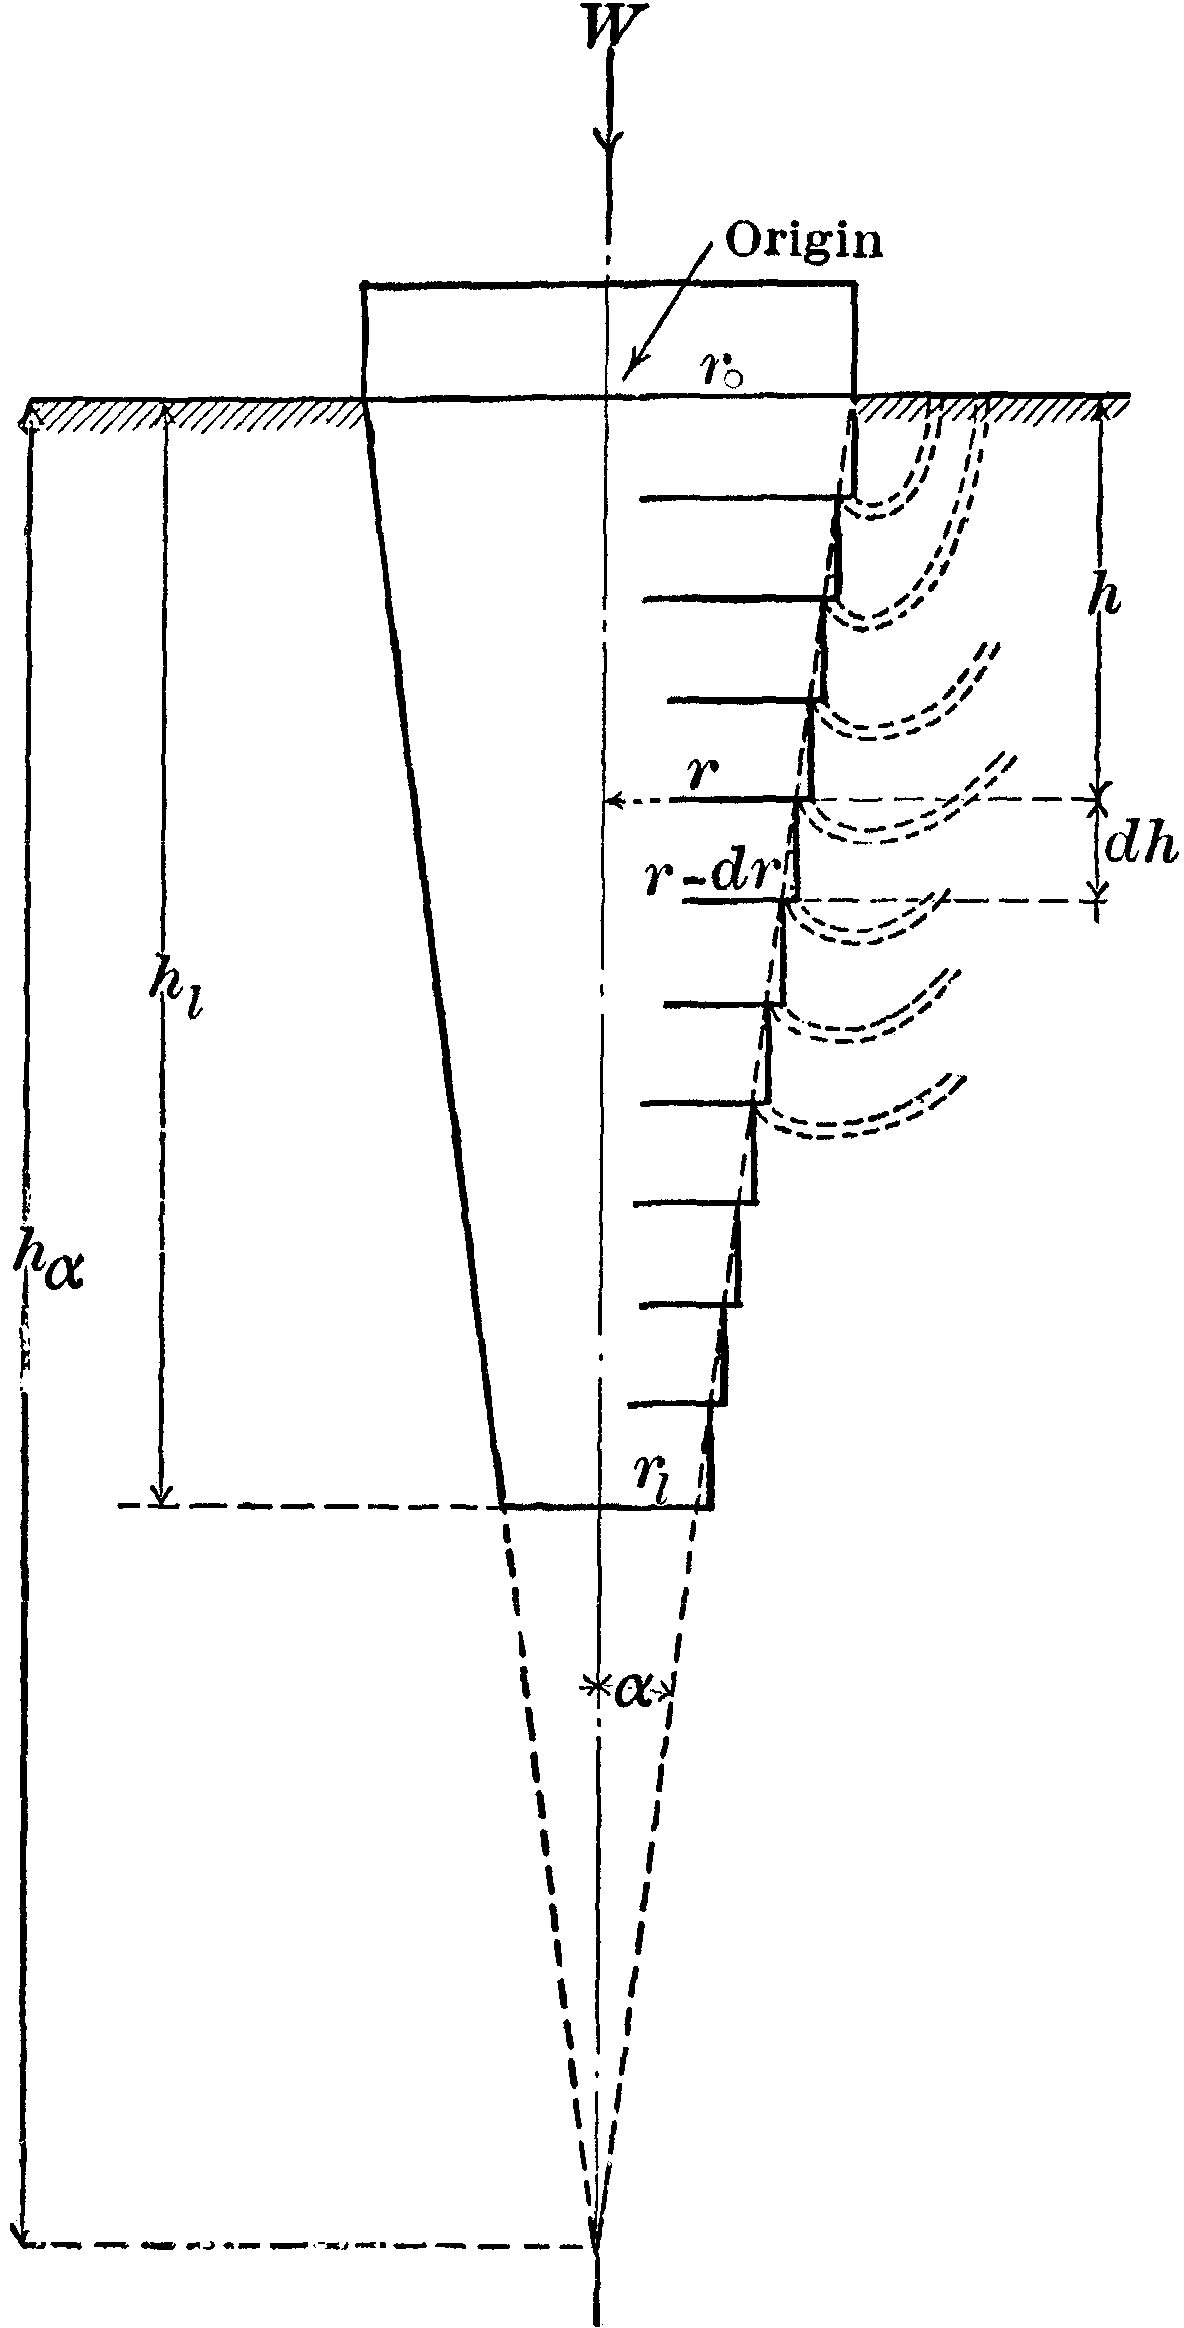
\includegraphics[width=.5\textwidth]{images/illus-417}
 \Legend{1}
\end{wrapfigure}
Consider a pulley-shaped foundation,
with data as indicated in \figref{1},
which, as in the case treated by
Desmond, may be a concrete or
timber pile jetted or driven to
place. Any form of cross-section
might be taken, but, for simplicity,
it is assumed as circular.

The dotted lines may be considered
to represent displacement
filaments passing out from the
horizontal rims to the free surface
around the head of the pile. The
position of these lines can only be
inferred from the treatises, say
Ketchum's or Vierendeel's, as few
if any precise investigations have
been made along this line.

At incipient motion of the pile,
it being assumed that it is at its
final depth, any increment of the
load will cause an actual displacement
of the particles, and this will
manifest itself as an increment
or surface displacement to the upheaval surface which has formed
around the head of the pile in driving. This assumption is necessary
under the Rankine hypothesis of incompressible particles,
although it has been the writer's experience that the phenomenon
is often difficult to observe at such a stage. The load at this
time is considered to be the ultimate carrying capacity, by the
Rankine law.
\PG--File: 418.png---\*******\************\*********\******\---------------

The area of a small rim of variable radius, $r$, and width, $dr =
2\pi r\, dr$.
\begin{align*}
   \text{Let } p
&= \text{the intensity of pressure on this rim element.}
\\
   \text{Then } p
&= wh\Bigl( \frac{1 + \Sin\phi}
                 {1 - \Sin\phi} \Bigr)^{\!2} \text{ for a maximum,}
\\
   \text{where } w
&= \text{the weight of a cubic unit of earth,}
\\
   \text{and } \phi
&= \text{the angle of internal friction, assumed as constant.}
\end{align*}

The total pressure on the element
$= 2\pi r\,dr \Bigl( \dfrac{1 + \Sin\phi}
                                {1 - \Sin\phi} \Bigr)^{\!2} wh$.
\begin{flalign*}
  \text{Now substitute } r &= (h_\alpha - h)\Tan\alpha,  &&\\
  \text{and }           dr &= -\Tan\alpha\,dh,  &&
\end{flalign*}
where $h_\alpha$ represents the distance from the surface to the vertex of
the cone formed by the surface of the pile, $h_l =$ the actual length
in the earth, and $\alpha =$ the angle of slope of the conical surface. The
total pressure on the rim element becomes
\[
  2\pi w \Bigl( \frac{1 + \Sin\phi}
                        {1 - \Sin\phi} \Bigr)^{\!2}
  \Tan^2 \alpha \int_{h_l}^0 -(h_\alpha - h) h\,dh.
\]

In order to take account of a principle of continuity, which in
this case will manifest itself in the law of pressure varying as a function
of the depth, one may conceive that, as the elementary rim pressure
exceeds the amount above given, the pile will tend to subside
under this, so that each rim will take its proportionate quota of
stress in turn. The total buoyant effect is at the limit when the
pulley-shaped foundation becomes a conical-shaped pile. The value
of the integral becomes:
\[
  \int_{h_l}^0 -(h_\alpha - h)h\,dh
= \Bigl[ -\Bigl( h_\alpha \frac{h^2}{2}
                       -  \frac{h^3}{3} \Bigr)\Bigr]_{h_l}^0
= h_\alpha \frac{{h_l}^2}{2} - \frac{{h_l}^3}{3} ,
\]
and, substituting this in the previous expression,
\[
  P_\text{(\textit{lat.})}
= 2\pi w \Bigl( \frac{1 + \Sin\phi}
                        {1 - \Sin\phi} \Bigr)^{\!2}
  \Tan^2 \alpha
  \Bigl[ h_\alpha \frac{{h_l}^2}{2} - \frac{{h_l}^3}{3} \Bigr],
\]
where the expression, $P_\text{(\textit{lat.})}$ represents the entire upward pressure
on the lateral surface of the pile. To this must be added the basal
pressure, giving, for the total load, $P$, which the pile can sustain
according to Rankine's theory:
\[
  P
= 2\pi w \Bigl( \frac{1 + \Sin\phi}
                        {1 - \Sin\phi} \Bigr)^{\!2}
  \Tan^2 \alpha
  \Bigl[ h_\alpha \frac{{h_l}^2}{2} - \frac{{h_l}^3}{3} \Bigr]
+ \pi {r_l}^2 w h_l \Bigl( \frac{1 + \Sin\phi}
                              {1 - \Sin\phi} \Bigr)^{\!2}.
\PGx--File: 419.png---\*******\************\*********\******\---------------
\]

In the case of the ``butt end down,'' the weight of the variable
column of earth may be similarly summed and added to the load
on the pile, and this equated to the bearing power of the base.

Such an analysis assumes, of course, that the earth conditions,
absence of cohesion, etc., will warrant a treatment by the Rankine
method. It is believed to give all that can consistently be demanded
of the hypothesis.

\textit{Limitations of the Theory.}---It will be seen that the above application
is quite limited in its efficiency as a working method. Specifically,
it neglects the friction on the vertical projections of the face.
Indeed, the Rankine premises do not take cognizance of any foreign
body, such as the pile, but confine the problem to an indefinite extent
of the material.

While it assumes the existence of displacement tubes, it makes
\begin{wrapfigure}{r}{.4\textwidth}
%[Illustration: \textsc{Fig.~2.}]
 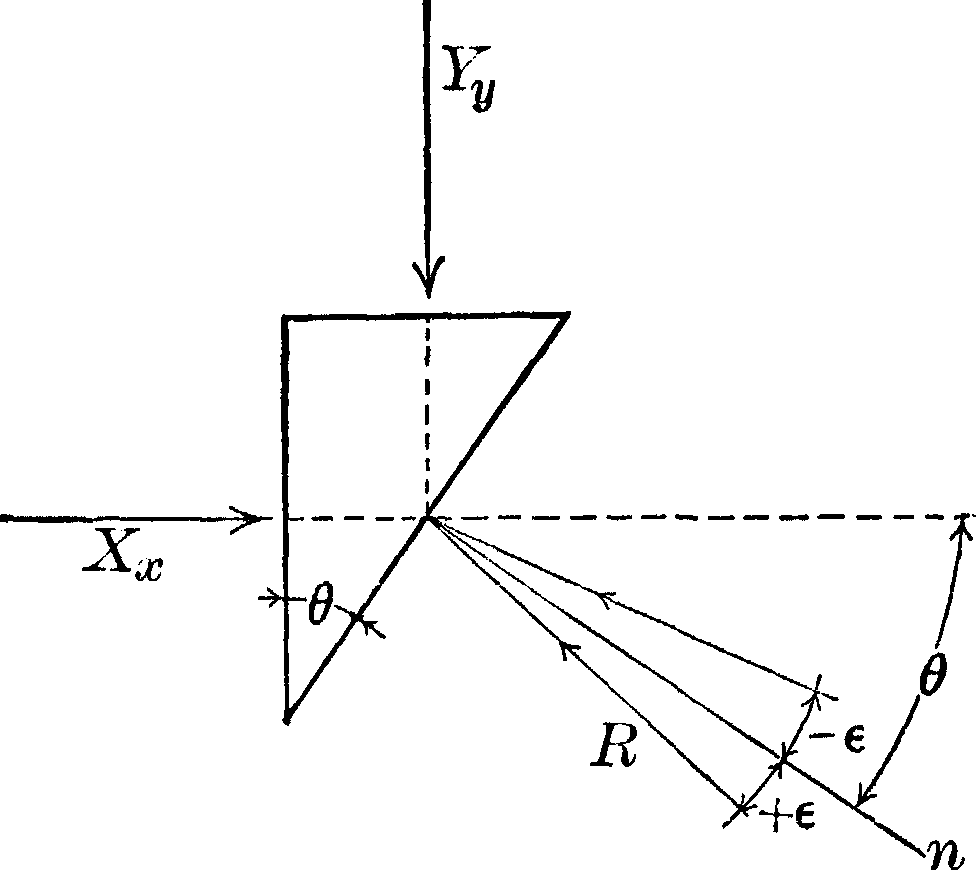
\includegraphics[width=.4\textwidth]{images/illus-419}
 \Legend{2}
\end{wrapfigure}
no analytical provision as to their zone
of action, unless one may take any series
of vertical and horizontal lines as defining
the field.

The usual applications of this theory
assume a constant coefficient of friction,
which, in the light of experiment, is only
approximately tenable; but, confining
the problem to its own more particular
domain, the chief limitation is the
necessity of the assumption of Moseley's law of least resistance as
Rankine referred to it, at once either the element of weakness or of
strength in his method, as one may prefer to call it.

Consider an ordinary wedge element of the material, \figref{2}, with
vertical and horizontal faces and an inclined face the normal of which,
$n$, is inclined at an angle, $\theta$, with the horizontal. The area of this
$\theta$-face may be conveniently taken as unity.

Let the intensity of the vertical stress be considered in this particular
case as due to a column of earth of length $y$ feet below the
surface of the ground, the value of which is $Y_{y}$. The corresponding
intensities upon the $x$- and $\theta$-planes, respectively, are $X_{x}$ and $R$.
The stress, $R$, has an obliquity of $\pm\epsilon$ from the normal. By compounding
stresses, by any of the elementary methods, there results the
general expression:
\PG--File: 420.png---\******\************\*********\******\----------------
\[
  X_x = \frac{\Tan\theta}{\Tan(\theta\pm\epsilon)}\, Y_y.
\]

To evaluate $X_{x}$, another condition is required. Rankine sought
to supply this condition through the Moseley assumption, taking the
obliquity, $\pm\epsilon$, as having its maximum value, $\phi$, at impending motion
of the particles. By seeking the maximum and minimum values of
$\dfrac{\Tan\theta}{\Tan(\theta\pm\epsilon)}$
on this basis, there results then, for the particular values
of $\theta$ where Rankine's value of $X_{x}$ may be assumed to hold:
\begin{align*}
  \theta &= \text{multiples of $\frac{\pi}{4} - \frac{\phi}{2}$, for $X_{x}$ a maximum,}
\\
  \theta &= \text{multiples of $\frac{3\pi}{4} - \frac{\phi}{2}$, for $X_{x}$ a minimum,}
\end{align*}
for positive values of $\phi$, and in a similar manner when $\phi$ is negative.
For example, taking a common value of $\phi = 30\degrees$, one receives
$X_{x} = \frac13 Y_{y}$ and $3 Y_{y}$, as in the ordinary case. For the above given
values of $\theta$, Rankine's solution may be considered to hold, but for
all other values the problem is absolutely indeterminate. The common
practice of engineers, in applying this method as a general solution
to problems of earthwork, is quite in keeping with that practice
which seeks the deportment of a column within the elastic limit from
tests to destruction.

Neither will the common defense, of the law being on the safe
side, hold in all cases. For instance, it has already been pointed out
by Boussinesq\footnote
 {``Essai th\'eorique sur l'\'equilibre des massifs pulv\'erulents, compar\'e
 \`a celui de massifs
 solides, et sur la pouss\'ee des terres sans coh\'esion,'' (1876), p.~5.}
that, in the case of a retaining wall when it is in
its ordinary position of equilibrium, otherwise than at the time of
incipient motion, as predicated by Rankine, although the particles
are less forcibly retained, they nevertheless exert upon the structure
a greater thrust than that given by Rankine.

A number of practical phases of this indeterminateness might be
cited, showing the shortcomings of the method as a theoretical device.
This is made apparent in the packing of balls. For example,
a rather low angle of repose may be expected for fine shot if it is
dropped from a short height, but had one the patience to arrange
the shot particle by particle in a pyramidal array, according to the
geometry of packing spheres, a much higher angle might be obtained
\PG--File: 421.png---\******\************\*********\******\----------------
for the slope of the pyramid, and this would be entirely independent
of the condition of the balls, that is, whether rough or frictionless.
Further, taking the old problem of the thousand 1-in.\ balls\footnote
  {Quoted by Greenhill from ``Cosmos,'' September, 1887,
  ``Hydrostatics,'' p.~52.}
packed
in cubical array in a $10$-in.\ cubical box, it is quite possible to conceive
of an angle of repose of $90\degrees$ if the sides of the box could be
gently removed, although, of course, in such a case, the equilibrium
would be very unstable. In the latter cases, the Moseley assumption
would be quite justifiable. However, taking another extreme, say,
the thrust of barrels on the walls of a warehouse, only the exigency
of an occasional earthquake could render the application of the
method theoretically permissible. The law is inoperative.

It is such limitations as have been cited that render the Rankine
method of rather doubtful utility for any general rational treatment,
either of the pile or the retaining wall. European and other than
American authorities have ceased treating the Rankine formula as a
general solution for all problems involving the lateral pressure of
earth, and prefer to give it its more proper position as defining
one particular kind of equilibrium. Even in its own special field,
a solution approaching nearer the facts may doubtless be secured in
many cases by the more determinate method of Greenhill,\footnote
  {Greenhill's ``Hydrostatics,'' pp.~45 \textit{et seq.}}
as in
the instance of barrel thrust.

\textit{Theoretical Position of the Method.}---In order, then, to give to
the Rankine theory applied to the pile that definiteness of position
which attaches, say, to that of Euler's formula in the column theory,
it may be defined as the theory of an infinitely smooth shaft afloat
on a medium deporting in several respects as a sort of generalized
fluid, where the particles are subject to negative normal stresses or
pressures and to tangential or friction stresses, but where no permanent
shearing resistance exists. In such a theory the vertical
pressures may be assumed to follow the hydrostatic law. The horizontal
pressures will also follow this law, but, owing to friction, the
effect is such as would occur with a reduced specific weight,
$w\Bigl( \dfrac{1\pm \Sin\phi}{1\mp \Sin\phi} \Bigr)$,
where $\phi$ is the angle of internal friction, or, as
Rankine referred to it usually, the angle of repose. The ($\pm$) signs
are to be used in the above for the case of maximum loadings, in
\PG--File: 422.png---\******\************\*********\******\----------------
which case the pressure exerted by the pile is a so-called ``active
force,'' as the term is used by Rankine. The ($\mp$) signs are for
minimum loads on the pile, namely, if the ``buoyancy'' of the surrounding
earth (viewing this now as an active force) is greater
than the load on the pile, as prescribed by this theory, the pile will
tend to rise, and may actually do so, especially if the medium contains
more or less water.

Accordingly, it will be seen that the laws of pulverulent masses
will agree well with the theory originally advanced by Boussinesq,\footnote
  {``History of the Elasticity and Strength of Materials,'' Vol.~II,
  Pt.~II, Article on
  Boussinesq, by Karl Pearson.}
and given later by Flamant,\footnote
  {``Stabilit\'e des Constructions,'' p.~111.}
Greenhill,\footnote
  {``Hydrostatics,'' pp.~45 \textit{et seq.}}
and others, in that they
are intermediate in their properties between fluids and solids. Fresh
cement, in its ordinary condition, will follow closely the hydrostatic
law, but, under pressure, will take on the properties of elastic bodies.
Even the Rankine equations, if consistently interpreted, find analogies
in the theory of stress and strain in solids on the one hand (Tresca),
and agree with the hydrostatic law for $\phi = 0$, on the other.

A dynamics of pulverulence is quite possible to formulate under
such a notion, and would probably find practical applications in designing
orifices for the discharge of grain, etc. Under this caption such
phenomena as have been described by Vierendeel\footnote
  {``Cours de Stabilit\'e des Constructions,'' Vol.~VI, p.~246.}
as occurring at the
circumference of disk piles, and by Le Conte\footnote
  {\textit{Transactions}, Am.\ Soc.\ C.~E., Vol.~XLII, p.~284.}
and Goodrich,\footnote
  {\textit{Transactions}, Am.\ Soc.\ C.~E., Vol.~XLVIII, p.~181.}
as
``cones'' and the like, forming under the bases of models, would probably
find interpretation as suppressed vortex or eddy effects.

\textit{Practical Utility of the Rankine Formula.}---While the Rankine theory
is little more than an abstraction, and if consistently and rationally
applied to a single pile can only be expected to give a fraction of the
real carrying power, its utility to the practicing engineer may still
exist in the fact that a multiple-pile system may be tested by Rankine's
equations about as logically as they may be applied to any ordinary
foundation. In such a multiple pile the integrity of the structure
is usually preserved by suitable framing; but, if this were not so, the
material in the cusp-like interstices between the piles can be expected
to be much more compressed, and consequently to have a considerably
\PG--File: 423.png---\******\************\*********\******\----------------
higher friction factor, than the less restrained material at the periphery
of the composite structure, thus tending to maintain this unity
of action.

In a multiple pile great reliance is placed on the increased density
of the soil, due to the driving, with the corresponding increase in the
friction coefficient. As the condensation under the Rankine premises
is purely inelastic, an approximate idea of the increase in density may
be found by an equation between the displacement of the pile and the
upheaval mass around the head.

Nearly all writers, with the exception of Vierendeel, in discussing
the bearing power of foundations, follow Rankine in ignoring the
stresses on the side walls, and confine their analysis solely to the base.
Accordingly, on the common theory, a designer of a multiple pile
would neglect the peripheral friction on the composite structure in
comparison with the presumably larger pressure on the base. In this
case such a procedure can be viewed as giving only crudely approximate
results. It is believed that the phenomenon of dilatancy of
media composed of rigid particles, as studied by Professor Osborne
Reynolds,\footnote
  {\textit{Philosophical Magazine} (London, E., and D.), Vol.~XX, 1885,
  p.~469. ``On the Dilatancy
  of Media Composed of Rigid Particles in Contact;'' also Reynolds'
  Works, Vol.~III.}
may even warrant the belief that this lateral friction is
larger than supposed, especially in water-bearing strata. The writer
will revert to this point later.

\textit{The Elastic Theory.}---Nearly all the structural problems of engineering
find their ultimate analysis in the elastic hypothesis. This
is true of the arch, and in a large measure of the retaining wall. Just
as the beam, on account of the labors of de St.\ Venant and his contemporaries,
owes its truly rational position to such elastic studies,
quite independent of the empiricists, the column theory, with of course
a few possible exceptions, may be said to have made no consistent
advances since the days of Euler by departing therefrom.

While to place such an apparently crude and sordid problem as the
pile in this field will undoubtedly seem inopportune, it is believed that,
in the end, such a step will avoid a great deal of useless effort and
incorrect thinking. It is thought important to bring out a few arguments
\emph{pro} and \emph{con} as to the advisability of such procedure.

In the first place, to make the problem of the lateral pressure of
earth truly determinate, the idea of strain is involved. Its introduction
\PG--File: 424.png---\******\************\*********\******\----------------
into the analysis is due to Boussinesq. Take the case previously
cited, of the problem of the balls packed in the 10-in.\ box in cubical
array. The problem of their lateral pressure against the walls owing
to their own weight becomes at least theoretically determinate, provided
all the stress and strain constituents of the material are known,
and the elastic deportment of the walls is understood. Although such
elastic solutions are in many cases extremely difficult to obtain, on
the other hand, they have the advantage of a high degree of certainty
of result, and will tend to obviate that endless modification so common,
say, in column and pile formulas.

As contributing data toward such a final and correct analysis, ideal
problems, approximating in part toward the actual conditions, may
be solved. For example, it may be shown that:
\begin{quote}
``If a vertical cylindrical hole of circular section is cut in a rigid
body, and an elastic cylinder of density $\rho$, which, if freed from the
action of gravity, would exactly fit the hole, is placed in it and stands
upon the bottom, \starellipsis\ the sides of the hole suffer the same
hydrostatic pressure as if it were filled with a liquid of density
$\rho (m - n) (m + n)$.'' (Ibbetson.)
\end{quote}

Slichter,\footnote
  {``Theoretical Investigation of the Motion of Ground-Waters,'' by
  C.\,S. Slichter
  (Government Printing Office, Washington, D.C., 1899), p.~333.}
in commenting along this line, remarks:
\begin{quote}
``It is important \starellipsis\ that we should have before us the solution
of as many problems as possible, since the most likely method by
which we shall be able to solve a new problem is by reducing it to one
of the cases in which a similar problem has been constructed by the
inverse process. Indeed, one must often be content to secure an
approximate solution in a given case by searching among problems
already solved for one whose equipotential lines or surfaces have a
form somewhat resembling the given boundary, and then so to modify
the problem by tentative methods as to produce conditions more nearly
corresponding to those of the given problem. For this reason it is
desirable to solve all possible kinds of problems \starellipsis\ whether
they seem to be `practical' or not.''
\end{quote}

Accordingly, Coulomb, Rankine, Weyrauch, Levy, Boussinesq,
K\"otter, and others, have contributed much in their study of various
kinds of equilibrium. The work of Boussinesq, while furnishing
valuable researches in the whole field, seems to be carefully ignored
by the practicing profession.

Such an elastic hypothesis, it has been urged, is less applicable to
\PG--File: 425.png---\************\************\*********\******\----------
the case of earth pressure than in the case of any other medium, it
being difficult to predicate continuity laws of the medium and the
existence of derivatives, as is done in hydrodynamic and elastic theories.
As sufficiently typical of such criticism, the remarks of Darwin\footnote
  {\textit{Minutes of Proceedings}, Inst.\ C.~E., Vol.~LXXI, 1883, ``On
  the Horizontal Thrust
  of a Mass of Sand,'' pp.~374 \textit{et seq.}}
are
closely to the point.
\begin{quote}
``It has always been assumed by previous writers that the tangential
action across an ideal interface in a mass of loose earth is of the same
nature as the statical friction between solids, and that when the tangential
stress has attained in magnitude a certain fraction of the
normal stress, the equilibrium is on the point of breaking down.
\starellipsis\ A little consideration will show that the hypothesis cannot
be exact, even with an ideal sand with incompressible grains, and
absolutely devoid of coherence. For imagine a mass of sand thrown
loosely together; then if the grains are of irregular shape a certain
portion of them will be resting on points and angles, thus occupying
more space than they might do.

``If the sand be now compressed, many of the grains will slip and
rotate, and fall into interstices; in fact a considerable amount of re-arrangement
will take place, and the density of the mass will rise
considerably---by quite 10 per cent.\ if the re-arrangement be thorough,
as found experimentally.

``Even if all the grains were spherical a considerable amount of
change would take place, and when they are angular of course much
more.~\starellipsis

``Hence it is clear that the coefficient of internal friction of sand
is a function of the pressure, and not merely of the pressure then
existing, but also of the pressure and shaking to which at some previous
period that portion of the mass of sand has been subjected.~\starellipsis

``It is quite impossible to say how much these causes will vitiate
any mathematical theory of the equilibrium of sand, but experience
seems to show that the vitiation is extensive.''
\end{quote}

On the other hand, in the elastic theory, the researches of Boussinesq\footnote
  {``Essai th\'eorique \starellipsis,'' p.~6.}
show that pulverulent material when under pressure---such as % original has "presure"
may occur in this particular case of the pile owing to impacted soil
through driving, even more than in the retaining wall---resists a change
of form with a force which is proportional to the mean of the three
principal stresses acting on the particle. He takes the coefficient of
rigidity, $\mu$, as varying with this mean pressure. As the weight on the
particle increases, either owing to its own ``head,'' or, in this case, to
\PG--File: 426.png---\*********\************\*********\******\-------------
the compressed soil in driving, the surrounding medium approaches an
elastic body in its properties. Under great pressure, of course, it
becomes perfectly so, thus justifying geologists or physicists in calculating
earth stresses, delta pressures, faults, etc., by known elastic
methods.

Now, the writer believes that there is a tacit notion, prevalent
among representative engineers, which is quite conformable to such an
hypothesis, and in support of this belief would quote the remarks of
Goodrich:\footnote
  {\textit{Transactions}, Am.\ Soc.\ C.~E., Vol.~XLVIII, ``Supporting
  Power of Piles,'' pp.~182 \textit{et seq.}}
\begin{quote}
``When a pile is supported entirely by the frictional resistance, the
actual region supporting the load is some deep ground level at which
the frictional resistance holding the pile has been transferred through
the earth in the shape of a conoid of pressure, the base of which gives
a total bearing value equal to the load and a unit bearing value which
the earth at that lower level will support. Each kind and degree of
compactness of earth will give a different angle for the slope of the
conoidal surface.''
\end{quote}

Again, he says:
\begin{quote}
``When supported by frictional resistance, they [the piles] must be
driven so far apart, or to such a depth, that the increased area of bearing
developed by the conoid of pressure having the required altitude
of frictional resistance meets a level which will afford the required
support before intersecting the conoid of a neighboring pile.''
\end{quote}

Such a description would seem to show analogies with the ``fan''
distribution of Stokes and Carus Wilson,\label{Wilson:fn:426}\footnote
  {\textit{Proceedings}, Physical Society of London, Vol.~XI, 1891,
  p.~194, ``The Influence of Surface-Loading
  on the Flexure of Beams.''}
with the local perturbations
of Boussinesq,\label{Boussinesq:fn:426}\multifootnote{Wilson:fn:426}{Boussinesq:fn:426}%
  {\textit{Proceedings}, Physical Society of London, Vol.~XI, 1891,
  p.~194, ``The Influence of Surface-Loading
  on the Flexure of Beams.''} %[** Footnote refers to same text as the last.]
or some of the equipollent effects of de St.\ Venant.\pagebreak % otherwise the wrapfigs to follow go haywire

It is natural to ask, however, how the inelastic distortions of
Darwin can be made to harmonize with the other views. The answer
would be by postulating or defining the medium. Slichter,\footnote
  {``Theoretical Investigation of the Motion of Ground-Waters,''
  p.~305.}
in a
somewhat related problem involving a study of the flow of ground-waters
through a soil, has attacked his problem very successfully by the
assumption of a mean soil. The size of the grains in a soil having
the same transmission power as the more complex soil he calls the
``effective'' size. He says:
\begin{quote}
``There probably exists a tendency in every such soil toward a
certain average size and mean arrangement of grains which the theory
\PG--File: 427.png---\*******\************\*********\******\---------------
of probabilities would justify us in setting up as an ideal soil to replace
a given soil in the investigation.''
\end{quote}

The same remarks may be applied to the analysis of the pile and
related phenomena. It is this idealization of the problem which is
tacitly done in all the problems of engineering, perhaps, however, with
less justification at this time in the theory of earth pressure, on account
of the lack of physical investigation.

On the whole, the opinion of elasticians, Darwin and de St.\ Venant
included, would seem to be favorable to an elastic analysis of the problem
of the lateral pressure of earth and pulverulent material. Pearson,\footnote
  {``History of Elasticity and Strength of Materials,'' Vol.~II,
  Pt.~II, pp.~313 and 357.}
in his critique of the elastic analysis of Boussinesq, has said:
\begin{quote}
``They appear to contain the most complete scientific theory yet
given of the stability of such a mass \starellipsis\ indeed, they are perhaps
the limit to what elastic theory can provide in these directions.''
\end{quote}

In view of the dearth of knowledge of strain and friction factors,
little progress can be made. It is believed, however, that as engineers
direct their attention to the static outlook and conduct experiments
along this line, a great many features now rather obscure will clear
up. Such a study also affords another angle of vision upon the pile
viewed dynamically and the retaining wall.

\textit{General Notions.}---For purposes of discussion, consider a pile
driven or jetted to place and carrying, say, its maximum load. It
is desired to investigate the mechanical state of the soil as it reacts
upon the pile and prevents its further subsidence under the load.
The principles of mechanics\footnote
  {``Theory of Elasticity,'' by Love, Chapter~V, pp.~122 \textit{et seq.}}
furnish the following well-known equations
for the static equilibrium of a volume element of the material
surrounding the pile, say, a small parallelopiped the co-ordinates of
which, as shown in \figref{3}, are $x$, $y$, and $z$.
\begin{align*}
  &\frac{\partial X_x}{\partial x}
+ \frac{\partial X_y}{\partial y}
+ \frac{\partial X_z}{\partial z} + \rho X = 0
\\
  &\frac{\partial Y_x}{\partial x}
+ \frac{\partial Y_y}{\partial y},
+ \frac{\partial Y_z}{\partial z} + \rho Y = 0
\\
  &\frac{\partial Z_x}{\partial x}
+ \frac{\partial Z_y}{\partial y}
+ \frac{\partial Z_z}{\partial z} + \rho Z = 0
\end{align*}

Using the Kirchoff notation, as preferable to that of Lam\'e, the
expression, $X_{x}$, represents the intensity of normal stress on the elementary
area, $dy\, dz$, of the parallelopiped, that is, the stress acting
\PG--File: 428.png---\******\************\*********\******\----------------
in the direction of the $x$-axis upon the plane element, $dy\, dz$, perpendicular
to this plane. Briefly, $X_{x}$ represents the $x$-stress upon the
$x$-plane. In a similar manner, $X_{y}$ is the $x$-stress on the $y$-plane, a shearing
or tangential stress; $Z_{z}$ is a normal stress upon the $z$-plane, and
so on. Since the shears at right angles are always equal, then $Y_{x} =
X_{y}$, $Z_{x} = X_{z}$,
\begin{wrapfigure}[17]{r}{.45\textwidth}
%[Illustration: \textsc{Fig.~3.}]
 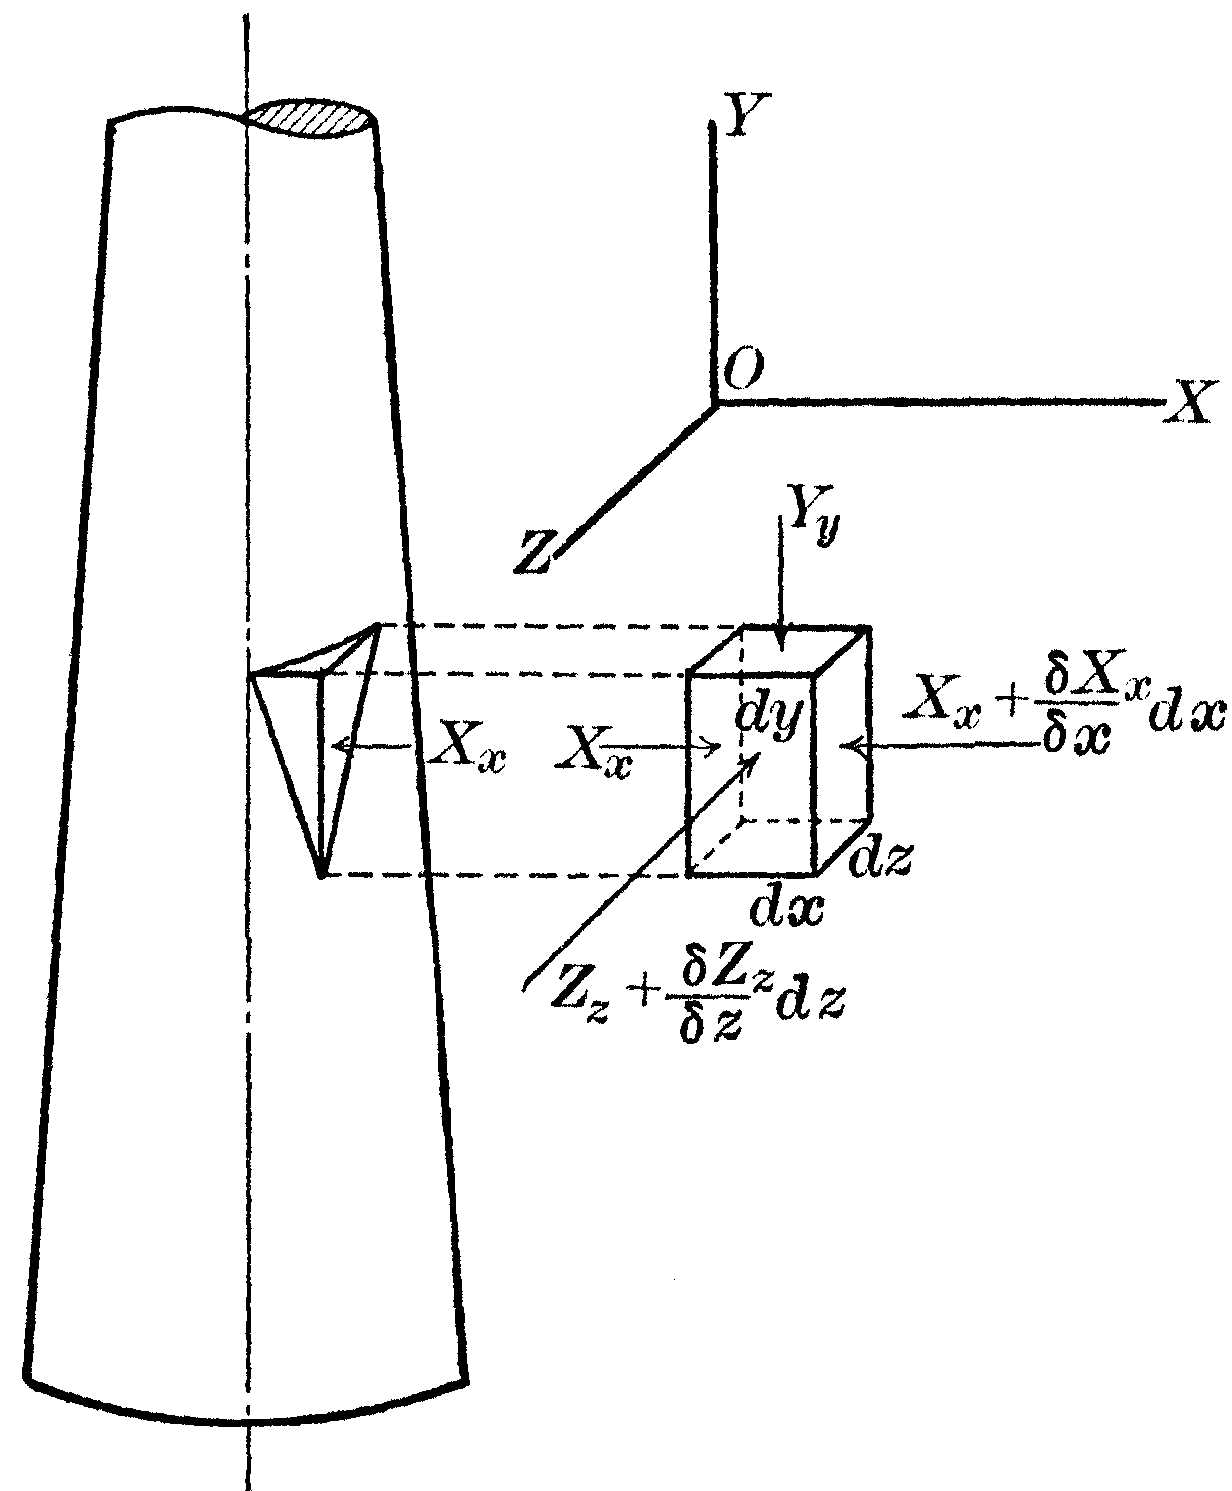
\includegraphics[width=.45\textwidth]{images/illus-428}
 \Legend{3}
\end{wrapfigure}
 $Z_{y} = Y_{z}$; but, for convenience of mental retention,
the symmetrical notation commends itself. The equivalence can be
asserted as desired in calculations of any particular problem.

The expressions, $\rho X$, $\rho Y$, and $\rho Z$, where $\rho$ is the density, represent
``body forces,'' such as gravity or ``centrifugal'' force. In this
case, these volumetric forces may be the components of gravity in the
direction of the co-ordinate axes,
or, as these are taken in \figref{3},
$\rho X = \rho Z = 0$, and $\rho Y =$ the
weight of the earth per cubic foot
in the engineer's notation. For
sand charged with water, this
would be, say, 110~lb., or as the
case might be.

The foregoing equations, as
used by Rankine\footnote
  {\textit{Philosophical Transactions}, Royal Society, 1857.}
in his original
paper, are rigid body equations.
Boussinesq,\footnote
  {``Essai th\'eorique sur l'\'equilibre d'\'elasticit\'e des massifs
  pulv\'erulents \starellipsis,'' p.~24, etc.}
by introducing a
comprehensive theory of strain,
formulates an independent system
for the theory of earth
pressure. There are, of course,
relations of compatibility in the general problem which will show
analytically, as already shown for the Patton equations, that the
engineer cannot choose his values at random.

Thus far, as the writer has discovered, few practical data in the
matter of strain are accessible for different earths. Reference to this
must be brief. The theory, then, will be founded on stress relations,
as in the ordinary beam formula, for practical purposes.

In the case of conical or cylindrical piles, the equations for static
equilibrium in a final analysis will be best expressed in the well-known
\PG--File: 429.png---\******\************\*********\******\----------------
cylindrical co-ordinates, the notation being similar to that used
before, namely:
\begin{align*}
& \frac{\partial Y_y   }{\partial y}
+ \frac{\partial Y_r   }{\partial r}
+ \frac{\partial Y_\phi}{r\, d\phi }
+ \frac{         Y_r   }{         r} + \rho Y = 0
\\
& \frac{\partial R_y   }{\partial y}
+ \frac{\partial R_r   }{\partial r}
+ \frac{\partial R_\phi}{r\, d\phi }
+ \frac{R_r - \phi_\phi}{         r} + \rho R = 0
\\
& \frac{\partial \phi_y}{\partial y}
+ \frac{\partial \phi_r}{\partial r}
+ \frac{\partial \phi_\phi}{r\, d\phi }
+ \frac{\phi_r + R_\phi}{         r} + \rho \phi = 0
\end{align*}

\begin{wrapfigure}[12]{r}{.45\textwidth}
%[Illustration: \textsc{Fig.~4.}]
 \vskip-12pt
 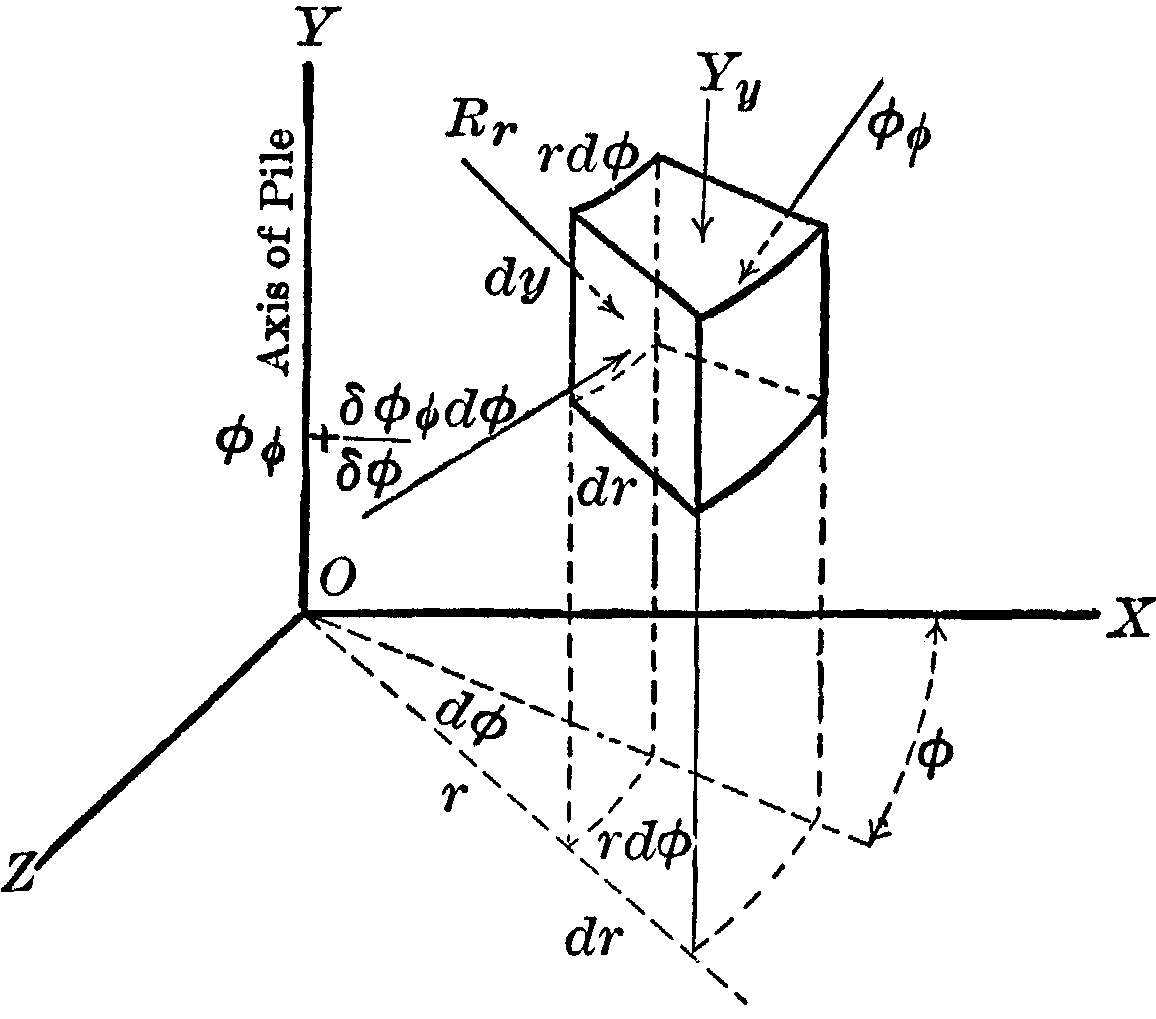
\includegraphics[width=.45\textwidth]{images/illus-429}
 \Legend{4}
\end{wrapfigure}
In these equations the capital letters give the direction of action of
the stress and the subscripts refer to the planes on which they act.
For example, $\phi_y$ represents the intensity in the direction of the normal
to the plane, $dr\, dy$, on the $y$-plane, that is, the plane, $dr\, r\, d\phi$, etc.
The shears in rectangular directions, as in the previous case, are equal.

In this more complicated case,
however, owing to the symmetry
about the $y$-axis, or axis of the pile,
the ``hoop compression'' becomes
constant around any particular
ring element of the radius, $r$. The
shears also vanish on the $\phi$-planes,
that is, any of the faces, $dy$, $dr$.
This distribution of stresses, when
a solution of the various particular
intensities is obtained, may ultimately
be used for obtaining the tubes of stress, their intensities and
slopes at any point, in the conoid described by Goodrich.

Now, to make any particular problem a determinate one, such types
of equilibrium equations as have been given are to be satisfied for
all values of the variables and for certain boundary conditions, namely,
at the upheaval surface and at the entire periphery of the pile. In
a continuous beam the analogy exists in the state at the supports.
Similarly, a correct column formula must not only satisfy such equilibrium
equations along the axis, but also hold for very long and very
short columns. The problem under discussion is relatively more
determinate than in the column problem, as the best that may ultimately
be expected in the latter case is a least-square solution.

At the surface of the pile the following type of equations must be
satisfied, as well as for the upper surface.\footnote
  {``Theory of Elasticity,'' by Love, Chapter~V, pp.~122 \textit{et seq.}}
\PG--File: 430.png---\******\************\*********\******\----------------
\begin{align*}
  X_n &= X_x \Cos(x n)
      + X_y \Cos(y n)
      + X_z \Cos(z n)
\\
  Y_n &= Y_x \Cos(x n)
      + Y_y \Cos(y n)
      + Y_z \Cos(z n)
\\
  Z_n &= Z_x \Cos(x n)
      + Z_y \Cos(y n)
      + Z_z \Cos(z n)
\end{align*}

To make these expressions clear, it may be remarked that the
surface of the pile, being in the general case the surface of a cone,
will transform the volume element of earth, $dx\, dy\, dz$ (\figref{3}), into
a tetrahedral element. And these equations assert the equilibrium
of all stresses on the tetrahedron in the directions, $x$, $y$, and $z$,
respectively.

Call the surface element of the pile, that is, the inclined face
of the tetrahedron element, the $n$-face, because its normal is, say, $n$.
Let its area be unity, for convenience of discussion. Then the other
faces, namely, the $x$, $y$ and $z$-faces, respectively, are $\Cos(xn)$, $\Cos(yn)$, and $\Cos(zn)$,
 where $(xn)$, $(yn)$, and $(zn)$ are the angles between
the $x$, $y$, and $z$-directions and the normal of the $n$-face or $n$.
Accordingly, $X_n$ is the resultant stress component in the $x$-direction
on the surface element of the pile. A similar set holds for the
ground surface, but becomes very much simpler owing to vanishing of
terms when the upheaval surface is assumed as horizontal.

Now, in a precise and finished analysis involving the strain relations,
both the boundary equations just given and the equilibrium
equations are usually expressed in terms of these strains. Just as
they are neglected in the derivation of the beam formula, they will be
neglected here. The two sets of equations will be used solely as stress
relations, as given, to keep the problem within working bounds.

A two-dimensional solution only can be attempted at this time,
on account of the analytical difficulties involved in the more general
treatment. It is believed, however, that a general solution exists in
the case where the ``immersed'' length of pile is zero in the Boussinesq\footnote
  {``Application des potentiels \`a l'\'etude de l'\'equilibre et du
  mouvement des solides \'elastiques,'' 1885.\\
  ``History of Theory of Elasticity,'' Todhunter-Pearson, Vol.~II,
  Pt.~II, p.~237.\\
  Love's ``Theory of Elasticity,'' Chapter~VIII.}
problem of the distribution of stress and strain due to a
rigid cylinder resting upon an infinite elastic solid, combined, of
course, with suitable superpositions to provide for the weight of
the soil. Moreover, since the strain in the earth at some distance from
the body is quite independent of the manner of distribution of the
peripheral stresses, but will depend rather on the resultant statically
\PG--File: 431.png---\******\********\*********\******\--------------------
equivalent to them, it is thought that this solution for immersion of
length zero may actually be taken for finite lengths of the pile.
It would seem to the writer that the existence of the ``cone'' under
the base will approximately justify this.

All authors, from Barlow and Rankine to the present time, have
pleaded a lack of experimental data with which to correlate their
mathematical investigations. The writer has felt this constraint in his
attempts to get any trustworthy results from the case given, after
analyzing the problem from different points of view; but, while these
efforts have been largely fruitless, they have afforded certain lines of
approach in analyzing the ``conoid.''

One of these is that, in the case of experiment, instead of restricting
the investigation solely to the special case of granular or pulverulent
media, as all engineers have heretofore done, the problem
should be generalized to include media which have elastic properties
within limits, say clay, hardpan, spongy soils, and very probably sand
in its most compact position, especially when it is charged with
water. It is believed that, eventually, when more experiments have
been made, these premises will be easier to work to than in the case
of granular media. In some preliminary experiments along this line,
made for the purpose of throwing light upon more precise efforts
to be undertaken, C.\,J.\ Green, Jun.\ Am.\ Soc.\ C.~E., and the
writer used rather fine and compacted saw-dust, in a duplication of the
Goodrich\footnote
  {\textit{Transactions}, Am.\ Soc.\ C.~E., Vol.~XLVIII, p.~181.}
experiment made with sand. Such a saw-dust medium will
permit a considerable magnification of the strain that may be expected
in an actual case, when a small vertical motion of the model
pile is made in the medium, keeping the ``pile'' close to the glass wall
of the box. Leygue,\footnote
  {\textit{Annales des Ponts et Chauss\'ees}, 1885.}
in his experiments on retaining walls, used
a series of strata of a different colored medium to bring out the faults
in the sand and confirm his notion of a curved surface for the interior
face of the Coulomb wedge. In like manner, this notion has been
tried by ``sprinkling'' a series of co-ordinate lines of any convenient
medium on the face of the glass wall when laid flat with the ``pile''
in place, and laying over this the saw-dust, with a view of showing
the strained lines when a small vertical displacement of the ``pile''
\PG--File: 432.png---\******\********\*********\******\--------------------
occurs. The original positions of the co-ordinates are marked on the
glass with a wax pencil.

Two limiting aspects are to be studied: First, the strained condition
for a very smooth or polished prism with a flat base, and then
that for one with serrated or notched faces next to the saw-dust. The
first case simulates that where the pressure on the sides is normal.
The second case approximates the actual status of a pile in a cohesive
soil where the full friction exists. While little of this has been carried
out, it is believed that qualitative data of value will be obtained by
using, not only straight prisms, but also wedges of rectangular cross-section
with the faces next the material inclined to and from the
vertical. It is hoped in the first case to obtain the deportment of the
material under the pile. Preliminary experiments seem to confirm,
partially at least, such a flow of stress as has been already derived
both experimentally and analytically by Hertz\footnote
  {Hertz, ``Miscellaneous Papers,'' Translation by Jones and Schott.\\
  Hertz, J.~F.\ Math. (Crelle), Bd.~92 (1881).\\
  Love's ``Theory of Elasticity,'' p.~195.}
in the well-known
problem of the pressure between two elastic bodies in contact. It is
thought, by carrying out the Goodrich experiment as thus described,
not only for sand, but also for other ``more springy'' media, that a
great deal of light may be afforded, not only on the basal action of
the pile, but also on the related problems of surface loading, as in
beams, etc. Here, analysis is already far ahead of experiment, at
least for elastic bodies.

In the second case, it is desired to discover the zone of action in
regard to the lateral friction in a cohesive and elastic soil. In the
subsequent analysis this can only be assumed for the case of pulverulent
material.

\textit{Two-Dimensional Stress Relations.}---With the Rankine premises
the uniplanar or two-dimensional case is easily extended to three
dimensions by the assumption of a vertical axis of symmetry, namely,
his ellipse of stress relation becomes an ellipsoid of stress; but, when
the influence of a body such as the pile is concerned, the problem
becomes greatly complicated, involving a solution in the case of stress
alone of the equations of equilibrium in cylindrical co-ordinates subject
to proper boundaries, as has been shown. The writer has been
unable to obtain general solutions for these, as has been already
remarked.
\PG--File: 433.png---\******\************\*********\******\----------------

It is proposed, in accordance with the suggestion of Slichter, to
attempt an approximate solution as the best available at this time.
Such a solution, accordingly, may be considered to be a second approximation
to that already given by Patton and by Desmond, but it will
avoid largely the Rankine inconsistencies. This may then be used
in studying the experimental data at hand with a view to discovering
the general law, if such law does not already exist, at least for
short piles in the Boussinesq problem of the rigid cylinder.\footnote
  {``Application des potentiels \`a l'\'etude de l'\'equilibre et du
  mouvement des solides
  \'elastiques,'' 1885 (Gauthier-Villars, Paris).}

\begin{wrapfigure}[11]{r}{.5\textwidth}
%[Illustration: \textsc{Fig.~5.}]
 \vskip-12pt
 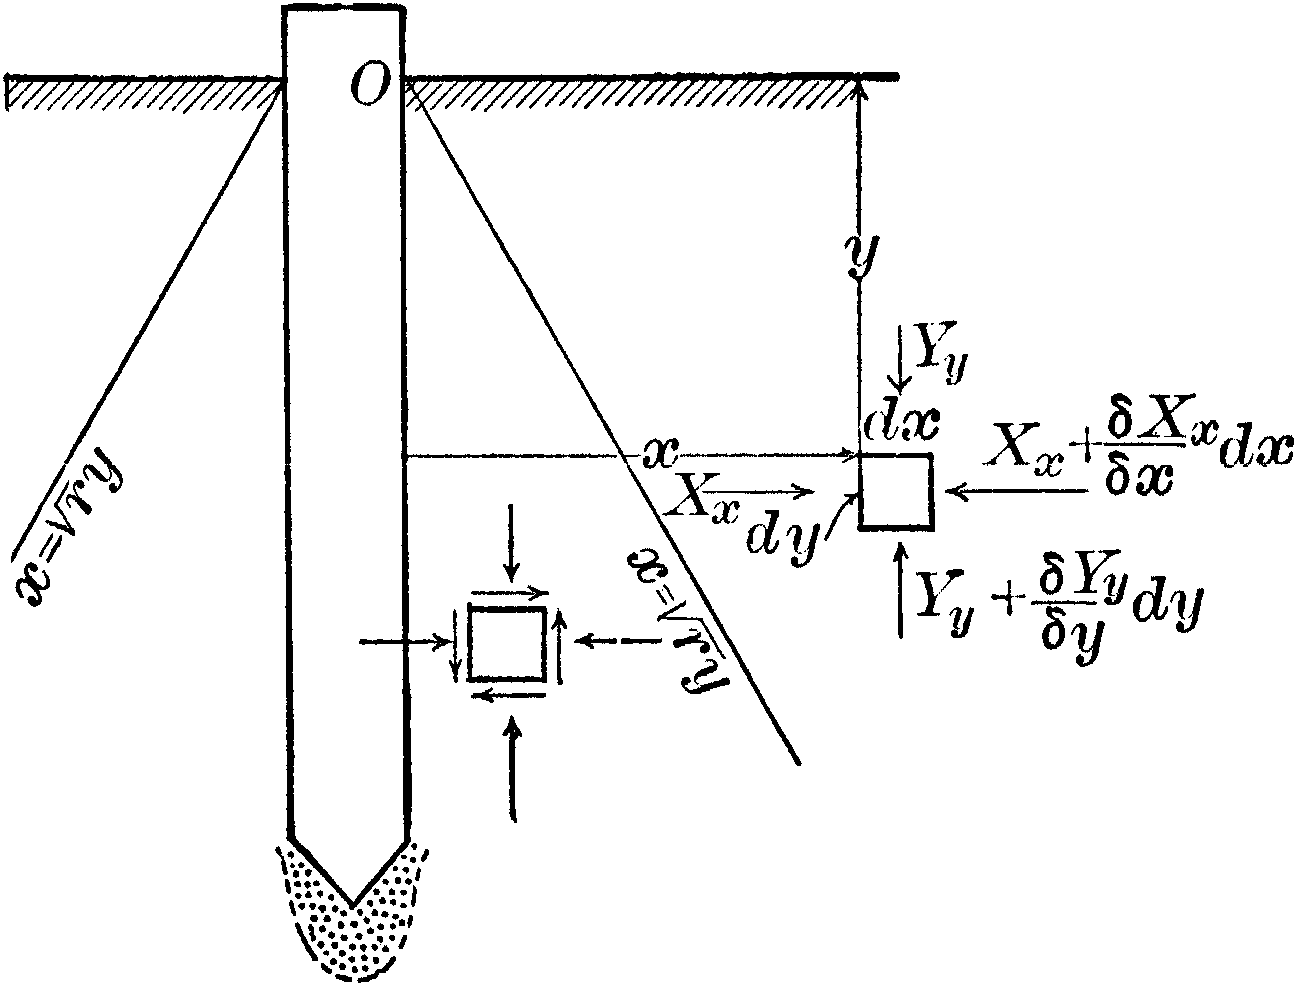
\includegraphics[width=.5\textwidth]{images/illus-433}
 \Legend{5}
\end{wrapfigure}
In a two-dimensional case, either of the sets of equilibrium equations
may be applied as it were to a pile of very large radius, or,
taking as equivalent, a stretch
of sheet-piling. Accordingly,
the piling partakes more or less
of the nature of the retaining
wall.

Two-dimensional treatments
of the equilibrium equations
have already been given, in the
case of the retaining wall, by
K\"otter\footnote
  {``Erddrucken auf St\"utzmauern,'' M\"uller-Breslau (Stuttgart, 1906),
  pp.~107 \textit{et seq.}}
and Boussinesq. As the
latter has discussed local effects
particularly, it is believed his results may be applied to the pile.\footnote
  {\textit{Annales des Ponts et Chauss\'ees}, T.~III, pp.~625--643.\\
  See also ``Theory of Elasticity,'' Todhunter-Pearson, Vol.~II,
  Pt.~II, p.~347; and
  \textit{Minutes of Proceedings}, Inst.\ C.~E., Vol.~LXV, p.~212.}

The equilibrium equations, being independent of $z$, or the direction
in the length of the wall or piling, reduce to
\begin{gather*}
  \frac{\partial X_x}{\partial x} +
  \frac{\partial X_y}{\partial y} = 0
  \text{ for the $x$-direction,}
\\
  \frac{\partial Y_x}{\partial x} +
  \frac{\partial Y_y}{\partial y} + (\rho y = w) = 0
  \text{ for the $y$-direction.}
\end{gather*}

The region of perturbation is supposed to extend to the line the
equation of which is
\[
  x = \sqrt{ \frac{1 - \Sin \phi}
                  {1 + \Sin \phi} } \,y = \sqrt{r} \,y,
\]
where the coefficient $\sqrt{r}$, is the square root of the Rankine
ratio. This
must here be tentatively assumed. (See \figref{5}.)
\PG--File: 434.png---\******\******\*********\********\--------------------

The general Rankine relation is assumed to hold outside of this
region at a distance from the pile, namely,
\[
\Sin^2 \phi  = \frac{(X_x - Y_y)^2 + 4X_y}{(X_x + Y_y)^2} \;,
\]
which states the expression for the ``stability of a mass of earth in
terms of the pressure at a point referred to any pair of rectangular
axes, $OX'$ and $OY'$, in the plane of greatest and least pressure.''\footnote
  {\textit{Philosophical Transactions}, Royal Society, Vol. 147, p. 18.}
Taking $4X_y = 0$, the common expression is easily derived.

As a justification of the use of the above, it is assumed here that
the plunger and cylinder experiments of Goodrich give a fair confirmation.
(Whether $\frac{1}{5\,000}$~in. $\pm$ movement of the ``plug'' will permit the
inference that the pressure on the plug is of the same intensity as that
on the walls of the cylinder has always raised a query in the writer's
mind.\footnote
  {\textit{Transactions}, Am.\ Soc.\ C.~E., Vol.~LIII, p.~283.})

Since the weight at the surface, assumed flat, is zero, the boundary
relations become, by the vanishing of terms in the equations for the
tetrahedron:
\[
Y = 0, \qquad Y_x =  X_y = 0.
\]
At the sheet-piling (the retaining wall in the problem of Boussinesq),
there results $X_y = \Tan \phi_1 X_x$, where $\Tan \phi_1$ is the tangent
of the angle of obliquity of the resultant pressure on the vertical face
at the pile.

Boussinesq assumes ``that in practice sustaining walls are generally
sufficiently rough to render a thin stratum of the pulverulent mass
stationary upon them. Hence the angle of friction between wall and
mass really reduces to the angle of friction of the pulverulent mass
upon itself.''\footnote
  {``History of Elasticity,'' Todhunter-Pearson, Vol.~II, Pt.~II, p.~336.}
This certainly is the maximum value. K\"otter differentiates,
however, the obliquity upon the $x$-face from that on the
$\theta$-face. In the case of sand, on account of dilatancy, the writer will
follow the Boussinesq assumption, but for soils not granular or pulverulent
will obtain such values for the later numerical computations
as may be had from actual tests. Cain, Darwin, and others
follow Boussinesq in retaining-wall design in this respect.
\PG--File: 435.png---\******\******\*********\********\--------------------

The following solution is given for the equations of equilibrium:
\begin{align*}
  X_x &= - \frac{1 - \Sin\phi}{1 + \Sin\phi}\, w y,\\
  X_y &= \phantom{-}   0,\\
  Y_y &= - wy,
\end{align*}
to apply without the region limited by $x - \sqrt{\dfrac{1 - \Sin\phi}{1 + \Sin\phi}}\, y$, and these are
the ordinary Rankine relations. Within this region, or in the zone of
perturbation of the pile, the following equations hold:
\begin{align*}
X_x &= -\frac{1 - \Sin\phi}{1 + \Sin\phi}\, \frac{(y+x \Tan\phi)w}{1+\sqrt{\dfrac{1 - \Sin\phi}{1 + \Sin\phi}}\Tan\phi}
\displaybreak[0]\\
Y_y &= -\frac{(y+x \Tan\phi)w}{1+\sqrt{\dfrac{1 - \Sin\phi}{1 + \Sin\phi}}\Tan\phi}
\displaybreak[0]\\
Y_x = X_y &= \frac{\Tan\phi_1\sqrt{\dfrac{1 - \Sin\phi}{1 + \Sin\phi}}
 \left(\sqrt{\dfrac{1 - \Sin\phi}{1 + \Sin\phi}}\,y - x \right)w}
{1+\sqrt{\dfrac{1-\Sin\phi}{1+\Sin\phi}} \Tan\phi}.
\end{align*}

In the above set of constituents, the stresses, $X_x$ and $Y_x = X_y$, are
induced stresses, that is, they are called into play on a hypothetical
infinitesimal motion outward of a retaining wall by the pressure head,
$Y_y$. In the Rankine language, they stand to each other in the relation
of ``cause to effect.'' The pressure head of earth is ``active,'' and
the induced lateral stress is ``passive.''

In the case of piling, however, $Y_x$ is the ``active'' stress. Accordingly,
one would assume, very consistently, that the resultant stress
on the $x$-face of a small element at the piling is active. To provide
for this case, one might proceed in the ordinary manner of Rankine,
namely, take $X \left(\dfrac{1 - \Sin\phi}{1 + \Sin\phi}\right)^2 \leqq Y_y$. This would appear to introduce
ambiguities into the problem. The writer will proceed as follows:

Call the passive or smaller ratio of Rankine $r_{p}$ and the active
or larger ratio $r_{a}$. If $Y_{x}$ and $X_{x}$ are active, it seems reasonable to
assume that the zone of perturbation due to pile action is larger. The
wedge defining this region, the slant height of which is $x = \sqrt{r}y$,
must intersect the head of the pile at the ground, because, whether
\PG--File: 436.png---\******\******\*********\********\--------------------
``active'' or ``passive,'' the shears vanish at the pile for $y = 0$. Let
$x = \dfrac{1}{\sqrt{r_p}}\,y=\sqrt{r_a}y$. The following is still true: At any point without
the region the general Rankine relations hold. The constituents hold
in general for all values of the variable within the region; the intensities
become zero at the surface; while, at the pile, for $\phi = 0$,
the ordinary Rankine relations still hold, the more general relations
hold for $\phi_{1}$.

To obtain a direct application of this, it is necessary to integrate
the intensity, $Y_{x}$, over the surface of the pile at $x = 0$. First call
\[
Y_{x0} = \Tan \phi_1 \frac{1+\Sin \phi}{1-\Sin \phi}\,
\frac{wy}{1 + \sqrt{\dfrac{1 + \Sin \phi}{1-\Sin \phi}}\Tan\phi_1}
= \frac{f r_a}{1 + f \sqrt r_a} w y
\]
for simplicity of expression, where $f =$ the coefficient of friction
at the pile, $w =$ the specific weight of the earth, and $y =$ the variable
depth. To apply this intensity in practice, where cylindrical and
slightly tapering piles are used, the assumption of Vierendeel and
the others is made, that the tangential intensity is independent of
the shape of the perimeter of the pile, a common enough assumption
in other branches of engineering.

By integration there results for a working formula comparable
with the Sanders' type in simplicity, but based on static considerations:
\begin{align*}
 W &= \frac{fr_a}{1 + f\sqrt{r_a}}\, w \pi D \int_0^L y\; dy, \\
\text{or }~W &= \frac{fr_a}{1 + f\sqrt{r_a}}\, w \pi D \dfrac{L^2}{2},
\end{align*}
where $\pi D$ is the mean circumference, $L$ is the length of pile, $w$ is
the weight of a cubic unit of earth, $f$ is the coefficient of friction, and
$r_{a}$ is the larger Rankine ratio, namely, $\dfrac{1+\Sin \phi}{1-\Sin \phi}$, $\phi$ being the
angle of internal friction, or so-called angle of repose.

Now $ w \pi D \dfrac{L^2}{2}$ is the normal hydrostatic pressure on a cylinder
for $w =$ specific weight.  Accordingly, $\dfrac{fr_a}{1 + f \sqrt{r_a}}$ is a more or less
rational friction factor for the same. While the formula is quite
\PG--File: 437.png---\******\******\*********\********\--------------------
as simple as Vierendeel's, it would seem to possess a more rational
derivation.

\textit{Effect of the Base.}---In the above working formula, upward pressure
on the base and sides, other than that due to tangential stresses,
has been disregarded as relatively negligible. This will need to be
discussed.

First, in the case of stiff earths possessing some elastic properties,
where a more or less well-defined ``conoid of pressure'' may
be assumed to exist, the pressure over the base of this conoid is
naturally assumed to be continuous. The principle of equipollent
loads (de St.\ Venant) shows that it is only in the region of the point
that the real distribution of stress has any effect. In the case of a
peg driven into a wooden beam and carrying a load on its head acting
longitudinally to the axis of the peg, the local effect of the stress
would be much the same whether the point of the peg entered a small
knot-hole or butted against sound wood. The assumption, then, will be
that the pressure under the pile is practically that which exists a foot
or two horizontally away. In the horizontal projection of the lateral
surface, the $Y_y$ is assumed to be that for $x = 0,$  $y = y_1$.

In the case of the Goodrich experiment, with the box and glass
walls, when the model pile is pushed down in the sand close to the
glass face the inverted paraboloid forming under the squared end
of the pile is only two or three end diameters of the pile in height.
The ``eddy'' action is largely confined to this small region. The
Rankine hypothesis, of necessity, assumes that the action is felt at
the surface, by reason of incompressible molecules arranged in most
compact space. It is believed, however, as has been shown by Bauschinger,
Darwin, and others, that considerable interstitial free space
exists in any pulverulent soil; accordingly, when the pressure occurs
it simply compacts the soil in the immediate region concerned.
The assumption, then, for semi-liquid materials, it would seem to be
reasonable, may be similar to that of the previous paragraph, namely,
that the pressure at the point and sides suffers no sudden breaks
or discontinuities from that a short distance away.

Accordingly, it is thought that the base and lateral buoyancy,
when the point is down, may be amply provided for by taking $L$ a
few diameters longer, say to the point of the inverted paraboloid,
instead of to the point of the pile, and using this length with the
\PG--File: 438.png---\******\************\*********\******\----------------
mean diameter of the pile. Such data, of course, would need to be
determined experimentally; or, perhaps it might be better to consider
the friction factor, $\dfrac{fr_a}{1+f\sqrt{r_a}}$, simply as an empirical parameter
to be determined for various cases.

\begin{figure*}[t] % table floated to get better pagination
\begin{center}\Small
\newlength\colheight
\def\tabcolsep{3.35pt}
\settowidth{\colheight}{Goodrich\quad }
\begin{tabular}{*{4}{r|} c|l| *{3}{r|} l}
\multicolumn{10}{c}{\textsc{\normalsize TABLE 1.---Annapolis Tests.}}
\\  \hline\hline
  \multicolumn{1}{c|}{
  \rotatebox{90}{\parbox{\colheight}{\centering Number.}} }
& \multicolumn{1}{c|}{
  \rotatebox{90}{\parbox{\colheight}{\centering Length.}} }
& \multicolumn{1}{c|}{
  \rotatebox{90}{\parbox{\colheight}{\centering Point.}} }
& \multicolumn{1}{c|}{
  \rotatebox{90}{\parbox{\colheight}{\centering Butt.}} }
& \multicolumn{1}{c|}{
  \rotatebox{90}{\parbox{\colheight}{\centering Hammer.}} }
& \multicolumn{1}{c|}{
  \rotatebox{90}{\parbox{\colheight}{\centering Fall.}} }
& \multicolumn{1}{c|}{
  \rotatebox{90}{\parbox{\colheight}{\centering Actual \\ test load.}} }
& \multicolumn{1}{c|}{
  \rotatebox{90}{\parbox{\colheight}{\centering Formula.}} }
& \multicolumn{1}{c|}{
  \rotatebox{90}{\parbox{\colheight}{\centering
  Goodrich \\ \rule{0pt}{4ex} $\dfrac{10 WH}{Sp}$}} }
& \multicolumn{1}{c}{\raisebox{4ex}{Remarks.} }
\\  \hline
\rule{0pt}{4.5ex}
  1 & 91 &  7 & 22 & 2\,300 & 22 &  75\,000 & 105\,200 &  96\,500
& $L = \Bigl\{\begin{matrix} 60 \text{ ft.~mud} \\
                   \phantom{0}6 \text{ ft.~sand}
       \end{matrix}\Bigr\} = 66$ ft.\null
\\
  2 & 91 &  7 & 22 &  ''   & 22 &  85\,090 & 133\,610 & 112\,000
& $L = \Bigl\{\begin{matrix} 60 \text{ ft.~mud} \\
                             12 \text{ ft.~sand}
       \end{matrix}\Bigr\} = 72$ ft.\null
\\
  3 & 73 &  9 & 18 &  ''   & $33\frac12$ & 34\,000 & 95\,450 & 67\,000
& $L = 61$ ft.~of mud
\\
  4 & 30 & 12 &  8 &  ''   & 22 &  38\,000 &  54\,400 & 84\,500
&\multicolumn{1}{c}{Sand.}
\\
  5 & 32 & 13 &  9 &  ''   & 22 & 110\,000 &  66\,500 & 168\,700
&\multicolumn{1}{c}{Sand.}
\\[3pt]  \hline\hline
\end{tabular}
\end{center}
\begin{quote}\small
For Cases 1, 2, and 3, $f = 0.1$ and $\phi = 15\degrees$ was used, for Cases 4 and 5, $f = 0.268 = \Tan\phi$,
and $\phi = 15\degrees$.

(See Patton's ``Civil Engineering,'' 1st ed., p.~487, for actual test for $f$ in liquid mud.)
$w$ is taken at 110~lb.\ per cu.~ft.
\end{quote}
\end{figure*}

\textit{Some Data.}---In lieu of any precise coefficients of friction and
angles of friction, no great precision can be expected in fitting the
formula to actual cases. In the following the formula has been applied
to the Annapolis\footnote
  {\textit{The Engineering Record}, May 11th, 1901; also
  \textit{Transactions}, Am.\ Soc.\ C.~E., Vol.~XLVIII,
  pp.~215 and 218.}
tests, J.\,P.\ Carlin, Assoc.\ M.\ Am.\ Soc.\ C.~E.,
\begin{wrapfigure}[7]{r}{.5\textwidth}
%[Illustration: \textsc{Fig.~6.}]
 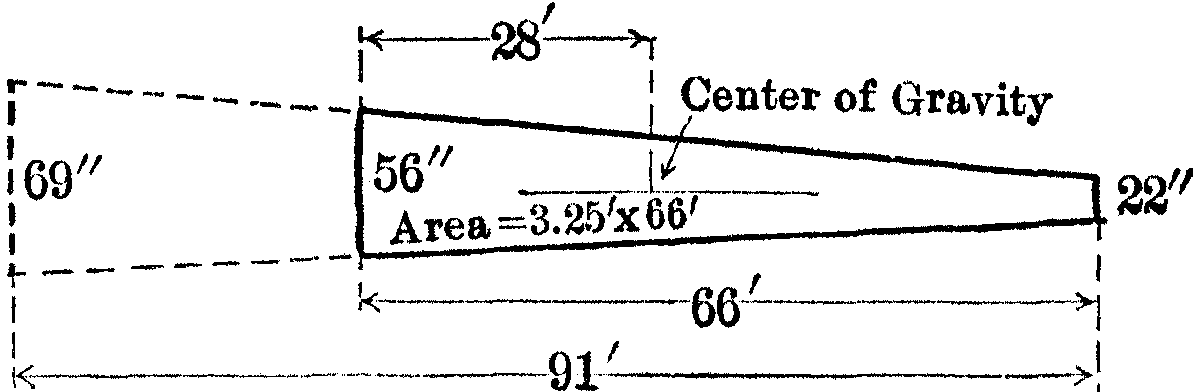
\includegraphics[width=.5\textwidth]{images/illus-438}
 \Legend{6}
\end{wrapfigure}
Engineer in Charge, also to the well-known Louisiana\footnote
  {Baker's ``Masonry,'' 8th ed., p.~247.}
pile (Proctorville,
La., 1856--57).

Case~1 is worked out below in
full, to show the effect of vertical
pressure on the side and base. The
developed surface of contact is a
trapezoid. The projected area on
a horizontal plane is 1.45 sq.~ft.
The area of the base is 0.267 sq.~ft.
\begin{alignat*}{2}
  \frac{1 + \Sin 15\degrees}
       {1 - \Sin 15\degrees} &= \frac{1.259}{0.741}\rlap{${} = 1.70$}  \\
  \sqrt{1.70} \times 0.1 &= 0.131 \\
\PGx--File: 439.png---\********\********\*********\******\------------------
  \frac{0.1\times 1.70}{1.131}
   \times 110\times 3.25\times 66\times 28
&= \phantom{9}99\,500, &&\text{friction on side,}\\
  \frac{66}{1.131} \times 110\times 0.267
&= \phantom{99}1\,700, &&\text{pressure on base,}\\
  \frac{28}{1.131} \times 110\times 1.46\phantom{0}
&=  \phantom{99}4\,000, &&\text{pressure on projected fa\rlap{ce,}}\\
\phantom{\frac99}  W &= \overline{\rule{0pt}{2.5ex}105\,200}, &~&\text{total calculated load.}
\end{alignat*}
The common hydrostatic methods of area multiplied by mean head
is used instead of the integration. The Rankine pressure on the
base and projected side is 5\,600 and 13\,000~lb., respectively, for
$\phi = 15$~degrees.\footnote
  {Note that 100~lb.\ instead of 110~lb.\ per cu.~ft.\ will give about
  10\,000~lb.\ smaller.}

For the Louisiana case, Baker's ``Masonry'' gives the following
data: Pile was 12~in.\ square throughout, driven 29.5~ft., and bore
29.9~tons without settlement. It settled slowly under 31.2~tons. The
same values of $f$ and $\phi$ are used as in Cases 4 and 5 of the Annapolis
test, namely, $f = 0.268$ and $\phi = 15\degrees$, or
\begin{alignat*}{2}
\frac{0.268\times 1.70}{1\times \sqrt{1.70}\times 0.268}
   \times 110\times 4\times \dfrac{29.5^2}{2}
&= 64\,800, &&\text{friction on sides,}\\
\frac{29.5}{1\times \sqrt{1.70}\times 0.268}
   \times 110\times 1.0^2
&= \phantom{6}2\,320, &&\text{pressure on base,}\\
\phantom{\frac9{\sqrt9}} W
&=  \overline{\rule{0pt}{2.5ex}67\,120}, &~&\text{total calculated load.}
\end{alignat*}

The static treatment presented gives an average deviation from
fact about commensurate with that of the most rational dynamic
formula. It is thought, however, that by obtaining actual experimental
factors, based on the physical qualities of the pile, a much
closer agreement would be possible. Most of the recorded data, being
made solely with reference to their availability for comparison and
study of dynamic formulas, omit such information.

The formula presented, being of the form of that given by
Vierendeel, who neglects the basal action, it should be easy, by drawing
tests, to ascertain the friction, expressed as a function of length % original has "acertain"
and mean diameter, for different soils.

\textit{Dilatancy of Granular Media.}---In his interesting discussion of
the Goodrich paper, the late Mr.\ Gould remarked:\footnote
  {\textit{Transactions}, Am.\ Soc.\ C.~E., Vol.~XLVIII, p.~214.}
\begin{quote}
``Another element which makes for safety, but which baffles calculation,
is the clinging action of the material through which the
\PG--File: 440.png---\*******\******\********\********\--------------------
pile is driven, and which action is set up immediately after it has
been allowed to come to rest. It is often impossible to draw a defective
pile even a very short time after it has been driven, unless a
few blows be given by the hammer to start it, when it may come up
very easily.''
\end{quote}

It is believed that the theory of the dilatancy of media composed
of rigid particles in contact, as proposed by Professor Osborne
Reynolds,\footnote
  {\textit{Philosophical Magazine} (London, E., \& D.), Vol.~XX, 1885, pp.~469 \textit{et seq.}; also
  Reynolds' Works, Vol.~III.}
will account for this phenomenon noticed and recorded
by many engineers. While the theory was formulated to account for
the sub-mechanics of the universe, not the least of its claims is that
it will place the theory of earth pressures on a true foundation. He says:

\begin{quote}
``I will point out the existence of a singular fundamental property
of such granular media which is not possessed by known fluids
or solids. \starellipsis\ I have called this unique property of granular
masses `dilatancy,' because the property consists in a definite change
of bulk, consequent on a definite change of shape or distortional
strain, any disturbance whatever causing a change of volume and
generally dilation.

``In the case of fluids, volume and shape are perfectly independent;
and although in practice it is often difficult to alter the
shape of any elastic body without altering its volume, yet the properties
of dilation and distortion are essentially distinct, and are so
considered in the theory of elasticity. In fact there are very few
solid bodies which are to any extent dilatable at all.

``With granular media, the grains being sensibly hard, the case
is, according to the results I have obtained, entirely different. So
long as the grains are held in mutual equilibrium by stresses transmitted
through the mass, every change of relative position of the
grains is attended by a consequent change of volume; and if in any
way the volume be fixed, then all change of shape is prevented.''
\end{quote}

The mathematics of this is long and difficult, in general. The essential
features, as it is desired to apply them in reference to Mr.\ Gould's
remarks, may be illustrated by the following experiment:

\begin{quote}
``If we have in a canvas bag any hard grains or balls, so long
as the bag is not nearly full it will change its shape as it is moved
about; but when the sack is approximately full a small change of
shape causes it to become perfectly hard. There is perhaps nothing
surprising in this, even apart from familiarity; because an inextensible
sack has a rigid shape when extended to the full, any deformation
diminishing its capacity, so that contents which did not fill
the sack at its greatest extension fill it when deformed. On careful
consideration, however, many curious questions present themselves.
\PG--File: 441.png---\*******\********\********\******\--------------------

``If, instead of a canvas bag, we have an extremely flexible bag of
india-rubber, this envelope, when filled with heavy spheres (No.~6
shot), imposes no sensible restraint on their distortion; standing on
the table it takes nearly the form of a heap of shot. This is apparently
accounted for by the fact that the capacity of the bag does not
diminish as it is deformed. In this condition it really shows us less
of the qualities of its granular contents than the canvas bag. But
as it is impervious to fluid, it will enable me to measure exactly
the volume of its contents.

``Filling up the interstices between the shot with water so that the
bag is quite full of water and shot, no bubble of air in it, and carefully
closing the mouth, I now find that the bag has become absolutely
rigid in whatever form it happened to be when closed.

``It is clear that the envelope now imposes no distortional constraint
on the shot within it, nor does the water. What then, converts the
heap of loose shot into an absolutely rigid body? Clearly, the limit
which is imposed on the volume by the pressure of the atmosphere.

``So long as the arrangement of the shot is such that there is
enough water to fill the interstices the shot are free, but any arrangement
which requires more room is absolutely prevented by the pressure
of the atmosphere~\starellipsis.

``The very finest quartz sand, or glass balls $\frac34$~in.\ in diameter, all
give the same results.''
\end{quote}

It would seem that such a state of affairs would tend to exist after
the driving, in the final rearrangement of the particles in granular
soils, and that the phenomenon may throw light on the case, as cited
by Mr.\ Gould. It would further seem to favor an elastic theory,
especially as one, to use another of Professor Reynolds' illustrations,
may note the firmness of a sandy beach after the recession of a wave,
in contradistinction to the quite fluid effect of the dry sand. The phenomenon
deserves to be studied in its relation to the pile.

The writer was led to appreciate the importance of the static point
of view, in the theory of the pile, through the suggestions of G.\,S.\
Williams, M.\ Am.\ Soc.\ C.~E\@. He was introduced to the Boussinesq
and K\"otter theories\footnote
  {A number of solutions involving different phases of this problem may
  be easily found.
  Among these the writer would call attention to a treatment of the
  glacier by Hopkins,
  Cambridge Phil.\ Soc.\ \textit{Transactions}, Vol.~8, 1849, in which
  he treats the glacier as an elastic
  body forcing its way between the walls of the valley, exerting
  lateral forces and friction on
  the sides of the stream quite comparable to the action of a pile in
  the earth. The Boussinesq
  literature, however, affords the most suggestion in addition to that
  of K\"otter.}
by Professor Alexander Ziwet. In making
acknowledgment to these authorities and to Professor A.\,B.\ Pierce for
discussion and criticism of these theories, the writer does not wish to
be construed as committing them to these views.
\PG--File: 442.png---\******\************\********\********\---------------

\clearpage
\chaptermark{Discussion: Ultimate Load on Pile Foundations}
\begin{center}
\Large\textbf{D\;I\;S\;C\;U\;S\;S\;I\;O\;N.}

\rule{.2\textwidth}{.4pt}
\end{center}

\textsc{Luther Wagoner, M.~Am.\ Soc.\ C.~E.}\speaker{Mr.\ Wagoner.} (by letter).---The writer
believes this to be a timely paper, and that, with sufficient data
concerning the physical properties of the resisting media, it will be
possible to construct a satisfactory formula for computing the safe
bearing load of a pile by purely statical methods. The assumption of
uniform values of the angle, $\phi$, is probably incorrect, and in what
follows the writer will consider a soil composed of mud to an
indefinite depth. The top layer of such a mud offers but little
resistance to penetration, and the resistance appears to increase more
rapidly than that of the static pressure due to depth. In tests made
by the writer in Islais Creek, which is an arm of San Francisco Bay,
the top mud is seen to be full of blow-holes, and relatively there is
much water to each unit of solid. A sample of the material taken
at a depth of 10~ft., or 15~ft.\ below mean tide, weighed 105~lb.\ per
cu.\ ft. When dried at steam heat it lost 34\% of its weight, or 35.7~lb.\
of water per cu.\ ft., which left 0.428~cu.\ ft.\ of volume for 69.3~lb.\ of
solids, or $\dfrac{69.3}{0.428} = 162$~lb.\ per cu.\ ft.\ for the weight of the solid
material, which is about the weight of the rock from which the mud
is derived.

From the foregoing this important deduction can be made: The
mud is the d\'ebris of rocks, in an exceedingly fine state of subdivision,
mixed with some clay. Any unit of this material possesses an
enormous surface as compared with its volume, and to this surface
the water is held by capillary action. Both the water and the separate
units of the mud are practically incompressible. The mixture is also
incompressible, and as long as it is saturated it must continue to
behave as an imperfect fluid. For example, a pile driven into such
material does not compress the soil laterally to any extent, but elevates
the soil near the pile. A blanket of rock or earth can be floated upon
the mud, and there will be little or no subsidence if the lateral flow
can be prevented by retaining walls, or, if a flat enough slope is given
to the mud thus covered it will stand. A sharp distinction must be
made for soils above and below the permanent ground-water level;
in the first case, the soil has voids, once occupied by water, and is
compressible by pile-drivers, and it is in such cases that a conical
pile gives good results. In the second case, there can be no compression,
but there is an upward displacement.

The mass of mud\speaker{Mr.\ Wagoner.} may be thought of as made up of small flattish
particles of solids, arranged, as a rule, nearly level, and the interstitial
space filled with water, or as a solid having an infinite number of
capillary tubes of variable diameters. It is obvious that under sufficient
\PG--File: 443.png---\******\************\********\********\---------------
pressure the water will move laterally through the tubes, and the
solids will be brought closer together, at the same time, the diameters
of the tubes will be reduced, and a greater head or pressure will be
required to produce further flow; but, as compression ensues, and the
diameters of the tubes are reduced, the rate of subsidence must
become slower; and, if for total subsidence we take $y$, and for time $x$,
it is clear that the resulting curve must be an asymptote to the
$x$ axis.

That the above is sound reasoning is borne out by various known
settlements, during long periods of time, where structures have been
founded upon clay or muds. In San Francisco a notable example of
settlement has occurred: A roughly semicircular body of land, one
mile long and half a mile wide, was reclaimed from the bay, and
upon this the business section of the city is built. A sea-wall, made
by dumping rock into a dredged trench, marks the outer boundary.
Inside of the sea-wall the streets have sunk slowly below grade, while
adjacent buildings upon long piles have remained intact; a total
subsidence of several feet, perhaps from 5 to 8~ft., has taken place in
the past thirty years. The subsidence of the sea-wall has been very
small in amount, certainly not greater than one-tenth of the landward
subsidence. This appears to the writer to be a case of steady loading
causing the water to percolate slowly seawards, thus allowing settlement
to occur.

S.\,W. Hoag, Jr., M.~Am.\ Soc.\ C.~E., in testing the soil for the Chelsea
Docks, New York City, where the mud is 180~ft.\ deep, drove four
groups of four piles each to a penetration of 50~ft., loaded each group
with concrete blocks, and noted the rate of subsidence. The experiment
ended at $51$ days, but the curves of subsidence show a total movement
of from $1\frac12$ to 3~in.\ where the load was 18 tons on a plain pile
and 34.6 tons on a lagged pile. The curves mentioned above are
markedly asymptotic to the time axis. These experiments deserve careful
study by any one desiring data regarding the behavior of piles in
a mud soil.\footnote
  {Report to John A.~Bensel, Engr.\ in Chief, N.~Y. Docks, Nov.\ 24th, 1902.}

It should not be forgotten that a formula may give correctly the
immediate or present ultimate bearing load of a pile, and yet serious
damage may arise from slow and long-continued settlements; and
it is the writer's belief\speaker{Mr.\ Wagoner.} that the attention of the investigator should
be turned toward the physics of the soil; thus, probably in a rational
formula, he will be able to forecast settlement as well as immediate
loads.

\textsc{John H. Griffith, Assoc.\ M.~Am.\ Soc.\ C.~E.}\speaker{Mr.\ Griffith.}---Since this paper
was printed, the writer's attention has been called to the fact that,
in the Annapolis tests, by Mr.\ Carlin, some of the piles had several
\PG--File: 444.png---\******\************\********\********\---------------
feet of water above the top surface of the earth surrounding them.
In a more general treatment, such a case should be considered, that is,
the boundary relation at the surface should be satisfied for the head
of water existing, instead of zero, as in the case worked out. If the
different strata of soil are considered, this will complicate the problem
still further.

At the time of this criticism, the writer made some approximate
calculations modifying the result for Case 1 which would indicate
that the water pressure would cause an increase in the value given
for this pile of about 10\,000 to 12\,000~lb.

In a practical theory, it will be necessary to assume a homogeneous
or isotropic soil medium, as has been done heretofore in engineering
studies of earth pressure; also to adhere to the common assumption
of an upper surface free from stress, as this will apply to the greater
number of cases in experience. Otherwise, it will be necessary to
increase the specific weight of the earth a proportionate amount, or
actually modify the stress constituents. All the problems of engineering
are really beyond the realms of analysis in the rigorous aspects,
and it is only by defining the media specifically, or averaging the
conditions, that practical solutions may be effected.

Another point has been raised, regarding the weight of the pile, or
dead load, which did not appear in the calculations. Since it has been
remarked to the writer that the specific weight of yellow pine or oak
when soaked with water may even exceed that of water, so that such
timbers will sometimes sink below the surface, the dead load will
compensate the value given in the first criticism to the amount of
several thousand pounds.

By far the most important factor in an elementary static analysis
is the question of friction and internal angle of friction. The writer
believes that in the main the experimental methods of approach heretofore
in vogue are often more or less unsatisfactory because based on
false premises of operation. Space will only suffice for one illustration
in the pile theory\speaker{Mr.\ Griffith.}, and that is the common notion advanced by
many engineers that the friction in drawing a pile is equal to that
encountered in driving it. This conclusion, if not absolutely erroneous,
is believed to be not true in general. The argument can only be
imperfectly stated, as follows: When the pile is driven the tubes of
stress will start out from the periphery of the pile and spread over
a correspondingly large area, probably in a conoidal distribution such
as has been well described by Goodrich. Assuming that a cohesive
material under pressure will be subject to the laws of elastic analysis,
such a notion would appear to be confirmed by the well-known tests
of Professors Carus-Wilson\footnote
  {\textit{Proceedings}, Physical Society of London, Vol.~XI, 1891, p.~194. Also Sir G.\,G. Stokes'
  works. A good discussion is in Bovey's ``Mechanics on Surface Loading of Beams.''}
on the beam for surface loading, and
\PG--File: 445.png---\******\************\********\********\---------------
of Marston\footnote
  {\textit{Transactions}, Am.\ Soc.\ C.~E., Vol.\ XXXII, pp.~99 and 273.}
for the roller problem, if the principle of equipollence is
strained a little from its usual applications. On the other hand, in
withdrawing the pile, such is not the case. One might indeed conceive
of the conoid as inverted, with its base at the free surface of earth, in
which case, for the pulverulent material, the friction on the periphery
would be equated to the weight of the material under discussion.

The treatment of Patton will illustrate this point in the fact that
he uses equations for minimum and maximum loadings, respectively,
taking $\dfrac {1 - \Sin \phi} {1 + \Sin \phi}$ for the minimum and
 $\dfrac {1 + \Sin \phi} {1 - \Sin \phi}$ for the maximum
lateral factor, according to Rankine. Now, if the pile is being
driven, the $\dfrac {1 + \Sin \phi} {1 - \Sin \phi}$ is operative while
 $\dfrac {1 - \Sin \phi} {1 + \Sin \phi}$, the reciprocal,
holds if for any reason the pile tends to rise. Accordingly, assuming
the coefficient of friction to be the same, as in the ordinary cases in
other fields of engineering, the total friction on the pile in the case
of withdrawal is less than that in driving. But, for a cohesive soil,
it would naturally be expected that a closer agreement would hold
between the two cases.

From the discussion by Mr.\ Gould on the paper by Mr.\ Goodrich,
quoted previously, the writer would be led to infer that a considerable
arching action of the ring elements around the pile, which are subject
to hoop compression, exists; and, after the pile moves upward, it
encounters little resistance, due to the earth friction, by reason of this;
but, whether the friction at the start in withdrawal is equal to that
in driving\speaker{Mr.\ Griffith.}, opens a path for discussion by the profession. It is hoped
that engineers who have the opportunity to withdraw piles may compare
their results with the loading the pile previously carried, or was
supposed to carry.

The whole static problem would appear to be a more general statement
of the problem usually ascribed to Cerruti and amplified in its
various phases by Boussinesq, Hertz, and various mathematicians,
viz.:

When an elastic cylinder or cone of revolution, initially free from
stress, is inserted in an elastic medium of relatively large extent, the
upper surface of which is flat or nearly so, and normal to the axis,
what are the strains and stresses in both due to vertical loading of the
cylinder?

For the practical purposes of the engineer, he will specialize this
problem to the case of a rigid pile and a pulverulent medium, and
ignore the discontinuity at the base for a first approximation. Professor
Burr, in his ``Mechanics of Materials,'' has given a derivation of
the equations of equilibrium in cylindrical co-ordinates which will be
\PG--File: 446.png---\******\********\********\********\-------------------
more easily understood by the practical engineer than by attempting
the transformation of co-ordinates usually given in the treatises. The
tubes of stress may be considered to start from the surface of the
pile with an angle of inclination to the axis equal to the angle of
friction of the earth on the pile. The principal stress is co-axial with
this tube. It will travel downward and radially until ultimately the
integrity of the tube is destroyed and displacement of the particles
takes place at some distance from the pile, in conformity with the
Rankine analysis.

The Rankine equations will satisfy the equations at a distance from
the pile, but cannot be assumed to hold locally on account of the
tangential or friction stresses which must be distributed into the earth
around the pile. Hence a correction or parameter must be inserted in
the Rankine stress values, and the resulting values inserted in the
equations of equilibrium. The values of these corrections must be
those which are compatible with the conditions at the ground and at
the pile. The resulting constituents must hold for all values within
the region affected by the tangential stresses. What is this region?
The writer's experiments thus far have shown rather unsatisfactory
results. In the first approximation it will be natural to take the
region as limited by a cone, but this does not seem to give close
agreement with fact. The\cleanbreak % forced break because marginpar refuses to stabilise
matter deserves investigation\speaker{Mr.\ Griffith.} by those
interested in placing the pile on a rational basis, where it belongs.

The writer has followed Mr.\ Wagoner's discussion with interest.
His citation of experiments for getting the specific weight, etc., of a
soil in its ocean bed is quite pertinent at this time.

With regard to the friction angle, the writer is prepared to agree
that the assumption of ``uniform values'' of this is not rigorous, as
has already been intimated by various investigators, say, Darwin and
Wilson; but, for the purposes of the practical engineer, it must be
assumed as constant for any particular medium, for reasons of
expediency. Such expressions for the variation of the coefficient of
friction, as have been given heretofore, are too complicated to introduce
into the theory in the early stages of its evolution, but must
ultimately find a place in a rational analysis of earth pressure. Most
engineers will be content if they can approximate to the true status
of loading, with a probable error of, say, $15$ or $20$\%~$\pm$, such as one
might expect in good bridge design.

The discussion of time rate of strain variation, involving questions
of subsidence, soil viscosity, etc., enters a comparatively virgin field
of study and experiment. Such investigations, considered in connection
with Slichter's studies, already cited, will undoubtedly receive an
important place in a final analysis of the pile, from the static point
of view.
\PG--File: 447.png---\******\************\********\********\---------------
\goodbreak
\begin{center}
\textsc{Summary.} % really a subsection
\end{center}

The practical points which are brought out in this paper are as
follows:

\textit{a.}---Attempts to get at the loading on a pile by a dynamic theory
are indirection of effort. The direct method is static, and should carry
out the work inaugurated by Patton, Vierendeel, Desmond, and others.
Both methods will co-operate in fixing load limits, and will serve as
check operations.

\textit{b.}---Their methods, while not rational of form, give an efficient
means of first approximation. Their value may be augmented in
efficiency by abandoning the Rankine ratio altogether and replacing by
a constant, which constant is to be selected on the basis of actual
tests from ultimate loads for similar soils, or from drawing tests when
properly interpreted. Using this constant with the ``hydrostatic
pressure''\cleanbreak % forced break because marginpar refuses to show on correct side of page
due to earth, a simple integration\speaker{Mr.\ Griffith.} gives the real load value
empirically when multiplied by the coefficient of friction; or, more
directly, owing to the uncertainty of this coefficient, it may be included
in the determination of the constant.

\textit{c.}---The notion of using the full Rankine pressure on the base is
probably in error, except for short piles and shallow foundations. The
Vierendeel form of neglecting this in comparison with that on the
periphery would seem to be more favorable to fact in a continuous
medium. This does not apply to a discontinuity at the base such as
would be implied by a rock foundation under the pile.

\textit{d.}---The pile is susceptible to an elastic treatment to a considerable
extent. Engineers should determine the moduli of soils,
pulverulent, plastic, or other, just as in steel or wooden structures.
The fact of average values of moduli may apply as properly as it does
in concrete or wood.

\textit{e.}---The Rankine theory should ultimately be displaced in favor
of an elastic treatment, because, by reason of strain, viscosity, and
cohesion, it can never fit the facts.

\textit{f.}---The question of dilatancy should be studied in its relation
to the pile.

\textit{g.}---Those who are interested in the development of a correct theory
of the pile should preserve the physical data for a static analysis,
such as that of the pile periphery, its slope, and diameters, also the
soil data and stratification. It has been the writer's experience, in
attempting to correlate figures with facts, that most of this has been
rejected in the dynamic analysis.

% we *do* want the licence to start recto, to emphasise it is an addition
\cleartorecto
\pagestyle{licence}
\setlength\parskip{0pt}\raggedbottom
\phantomsection
\par
\begin{PGboilerplate}[\tiny]| 8pt for B5
End of the Project Gutenberg EBook of Transactions of the American Society
of Civil Engineers, vol. LXX, Dec. 1910, by John H. Griffith

*** END OF THIS PROJECT GUTENBERG EBOOK 25222 ***

***** This file should be named 25222-pdf.pdf or 25222-pdf.zip *****
This and all associated files of various formats will be found in:
        http://www.gutenberg.org/2/5/2/2/25222/

Produced by Juliet Sutherland, David Wilson and the Online
Distributed Proofreading Team at http://www.pgdp.net


Updated editions will replace the previous one--the old editions
will be renamed.

Creating the works from public domain print editions means that no
one owns a United States copyright in these works, so the Foundation
(and you!) can copy and distribute it in the United States without
permission and without paying copyright royalties.  Special rules,
set forth in the General Terms of Use part of this license, apply to
copying and distributing Project Gutenberg-tm electronic works to
protect the PROJECT GUTENBERG-tm concept and trademark.  Project
Gutenberg is a registered trademark, and may not be used if you
charge for the eBooks, unless you receive specific permission.  If you
do not charge anything for copies of this eBook, complying with the
rules is very easy.  You may use this eBook for nearly any purpose
such as creation of derivative works, reports, performances and
research.  They may be modified and printed and given away--you may do
practically ANYTHING with public domain eBooks.  Redistribution is
subject to the trademark license, especially commercial
redistribution.



*** START: FULL LICENSE ***

THE FULL PROJECT GUTENBERG LICENSE
PLEASE READ THIS BEFORE YOU DISTRIBUTE OR USE THIS WORK

To protect the Project Gutenberg-tm mission of promoting the free
distribution of electronic works, by using or distributing this work
(or any other work associated in any way with the phrase "Project
Gutenberg"), you agree to comply with all the terms of the Full Project
Gutenberg-tm License (available with this file or online at
http://gutenberg.org/license).


Section 1.  General Terms of Use and Redistributing Project Gutenberg-tm
electronic works

1.A.  By reading or using any part of this Project Gutenberg-tm
electronic work, you indicate that you have read, understand, agree to
and accept all the terms of this license and intellectual property
(trademark/copyright) agreement.  If you do not agree to abide by all
the terms of this agreement, you must cease using and return or destroy
all copies of Project Gutenberg-tm electronic works in your possession.
If you paid a fee for obtaining a copy of or access to a Project
Gutenberg-tm electronic work and you do not agree to be bound by the
terms of this agreement, you may obtain a refund from the person or
entity to whom you paid the fee as set forth in paragraph 1.E.8.

1.B.  "Project Gutenberg" is a registered trademark.  It may only be
used on or associated in any way with an electronic work by people who
agree to be bound by the terms of this agreement.  There are a few
things that you can do with most Project Gutenberg-tm electronic works
even without complying with the full terms of this agreement.  See
paragraph 1.C below.  There are a lot of things you can do with Project
Gutenberg-tm electronic works if you follow the terms of this agreement
and help preserve free future access to Project Gutenberg-tm electronic
works.  See paragraph 1.E below.

1.C.  The Project Gutenberg Literary Archive Foundation ("the Foundation"
or PGLAF), owns a compilation copyright in the collection of Project
Gutenberg-tm electronic works.  Nearly all the individual works in the
collection are in the public domain in the United States.  If an
individual work is in the public domain in the United States and you are
located in the United States, we do not claim a right to prevent you from
copying, distributing, performing, displaying or creating derivative
works based on the work as long as all references to Project Gutenberg
are removed.  Of course, we hope that you will support the Project
Gutenberg-tm mission of promoting free access to electronic works by
freely sharing Project Gutenberg-tm works in compliance with the terms of
this agreement for keeping the Project Gutenberg-tm name associated with
the work.  You can easily comply with the terms of this agreement by
keeping this work in the same format with its attached full Project
Gutenberg-tm License when you share it without charge with others.

1.D.  The copyright laws of the place where you are located also govern
what you can do with this work.  Copyright laws in most countries are in
a constant state of change.  If you are outside the United States, check
the laws of your country in addition to the terms of this agreement
before downloading, copying, displaying, performing, distributing or
creating derivative works based on this work or any other Project
Gutenberg-tm work.  The Foundation makes no representations concerning
the copyright status of any work in any country outside the United
States.

1.E.  Unless you have removed all references to Project Gutenberg:

1.E.1.  The following sentence, with active links to, or other immediate
access to, the full Project Gutenberg-tm License must appear prominently
whenever any copy of a Project Gutenberg-tm work (any work on which the
phrase "Project Gutenberg" appears, or with which the phrase "Project
Gutenberg" is associated) is accessed, displayed, performed, viewed,
copied or distributed:

This eBook is for the use of anyone anywhere at no cost and with
almost no restrictions whatsoever.  You may copy it, give it away or
re-use it under the terms of the Project Gutenberg License included
with this eBook or online at www.gutenberg.org

1.E.2.  If an individual Project Gutenberg-tm electronic work is derived
from the public domain (does not contain a notice indicating that it is
posted with permission of the copyright holder), the work can be copied
and distributed to anyone in the United States without paying any fees
or charges.  If you are redistributing or providing access to a work
with the phrase "Project Gutenberg" associated with or appearing on the
work, you must comply either with the requirements of paragraphs 1.E.1
through 1.E.7 or obtain permission for the use of the work and the
Project Gutenberg-tm trademark as set forth in paragraphs 1.E.8 or
1.E.9.

1.E.3.  If an individual Project Gutenberg-tm electronic work is posted
with the permission of the copyright holder, your use and distribution
must comply with both paragraphs 1.E.1 through 1.E.7 and any additional
terms imposed by the copyright holder.  Additional terms will be linked
to the Project Gutenberg-tm License for all works posted with the
permission of the copyright holder found at the beginning of this work.

1.E.4.  Do not unlink or detach or remove the full Project Gutenberg-tm
License terms from this work, or any files containing a part of this
work or any other work associated with Project Gutenberg-tm.

1.E.5.  Do not copy, display, perform, distribute or redistribute this
electronic work, or any part of this electronic work, without
prominently displaying the sentence set forth in paragraph 1.E.1 with
active links or immediate access to the full terms of the Project
Gutenberg-tm License.

1.E.6.  You may convert to and distribute this work in any binary,
compressed, marked up, nonproprietary or proprietary form, including any
word processing or hypertext form.  However, if you provide access to or
distribute copies of a Project Gutenberg-tm work in a format other than
"Plain Vanilla ASCII" or other format used in the official version
posted on the official Project Gutenberg-tm web site (www.gutenberg.org),
you must, at no additional cost, fee or expense to the user, provide a
copy, a means of exporting a copy, or a means of obtaining a copy upon
request, of the work in its original "Plain Vanilla ASCII" or other
form.  Any alternate format must include the full Project Gutenberg-tm
License as specified in paragraph 1.E.1.

1.E.7.  Do not charge a fee for access to, viewing, displaying,
performing, copying or distributing any Project Gutenberg-tm works
unless you comply with paragraph 1.E.8 or 1.E.9.

1.E.8.  You may charge a reasonable fee for copies of or providing
access to or distributing Project Gutenberg-tm electronic works provided
that

- You pay a royalty fee of 20% of the gross profits you derive from
     the use of Project Gutenberg-tm works calculated using the method
     you already use to calculate your applicable taxes.  The fee is
     owed to the owner of the Project Gutenberg-tm trademark, but he
     has agreed to donate royalties under this paragraph to the
     Project Gutenberg Literary Archive Foundation.  Royalty payments
     must be paid within 60 days following each date on which you
     prepare (or are legally required to prepare) your periodic tax
     returns.  Royalty payments should be clearly marked as such and
     sent to the Project Gutenberg Literary Archive Foundation at the
     address specified in Section 4, "Information about donations to
     the Project Gutenberg Literary Archive Foundation."

- You provide a full refund of any money paid by a user who notifies
     you in writing (or by e-mail) within 30 days of receipt that s/he
     does not agree to the terms of the full Project Gutenberg-tm
     License.  You must require such a user to return or
     destroy all copies of the works possessed in a physical medium
     and discontinue all use of and all access to other copies of
     Project Gutenberg-tm works.

- You provide, in accordance with paragraph 1.F.3, a full refund of any
     money paid for a work or a replacement copy, if a defect in the
     electronic work is discovered and reported to you within 90 days
     of receipt of the work.

- You comply with all other terms of this agreement for free
     distribution of Project Gutenberg-tm works.

1.E.9.  If you wish to charge a fee or distribute a Project Gutenberg-tm
electronic work or group of works on different terms than are set
forth in this agreement, you must obtain permission in writing from
both the Project Gutenberg Literary Archive Foundation and Michael
Hart, the owner of the Project Gutenberg-tm trademark.  Contact the
Foundation as set forth in Section 3 below.

1.F.

1.F.1.  Project Gutenberg volunteers and employees expend considerable
effort to identify, do copyright research on, transcribe and proofread
public domain works in creating the Project Gutenberg-tm
collection.  Despite these efforts, Project Gutenberg-tm electronic
works, and the medium on which they may be stored, may contain
"Defects," such as, but not limited to, incomplete, inaccurate or
corrupt data, transcription errors, a copyright or other intellectual
property infringement, a defective or damaged disk or other medium, a
computer virus, or computer codes that damage or cannot be read by
your equipment.

1.F.2.  LIMITED WARRANTY, DISCLAIMER OF DAMAGES - Except for the "Right
of Replacement or Refund" described in paragraph 1.F.3, the Project
Gutenberg Literary Archive Foundation, the owner of the Project
Gutenberg-tm trademark, and any other party distributing a Project
Gutenberg-tm electronic work under this agreement, disclaim all
liability to you for damages, costs and expenses, including legal
fees.  YOU AGREE THAT YOU HAVE NO REMEDIES FOR NEGLIGENCE, STRICT
LIABILITY, BREACH OF WARRANTY OR BREACH OF CONTRACT EXCEPT THOSE
PROVIDED IN PARAGRAPH F3.  YOU AGREE THAT THE FOUNDATION, THE
TRADEMARK OWNER, AND ANY DISTRIBUTOR UNDER THIS AGREEMENT WILL NOT BE
LIABLE TO YOU FOR ACTUAL, DIRECT, INDIRECT, CONSEQUENTIAL, PUNITIVE OR
INCIDENTAL DAMAGES EVEN IF YOU GIVE NOTICE OF THE POSSIBILITY OF SUCH
DAMAGE.

1.F.3.  LIMITED RIGHT OF REPLACEMENT OR REFUND - If you discover a
defect in this electronic work within 90 days of receiving it, you can
receive a refund of the money (if any) you paid for it by sending a
written explanation to the person you received the work from.  If you
received the work on a physical medium, you must return the medium with
your written explanation.  The person or entity that provided you with
the defective work may elect to provide a replacement copy in lieu of a
refund.  If you received the work electronically, the person or entity
providing it to you may choose to give you a second opportunity to
receive the work electronically in lieu of a refund.  If the second copy
is also defective, you may demand a refund in writing without further
opportunities to fix the problem.

1.F.4.  Except for the limited right of replacement or refund set forth
in paragraph 1.F.3, this work is provided to you 'AS-IS' WITH NO OTHER
WARRANTIES OF ANY KIND, EXPRESS OR IMPLIED, INCLUDING BUT NOT LIMITED TO
WARRANTIES OF MERCHANTIBILITY OR FITNESS FOR ANY PURPOSE.

1.F.5.  Some states do not allow disclaimers of certain implied
warranties or the exclusion or limitation of certain types of damages.
If any disclaimer or limitation set forth in this agreement violates the
law of the state applicable to this agreement, the agreement shall be
interpreted to make the maximum disclaimer or limitation permitted by
the applicable state law.  The invalidity or unenforceability of any
provision of this agreement shall not void the remaining provisions.

1.F.6.  INDEMNITY - You agree to indemnify and hold the Foundation, the
trademark owner, any agent or employee of the Foundation, anyone
providing copies of Project Gutenberg-tm electronic works in accordance
with this agreement, and any volunteers associated with the production,
promotion and distribution of Project Gutenberg-tm electronic works,
harmless from all liability, costs and expenses, including legal fees,
that arise directly or indirectly from any of the following which you do
or cause to occur: (a) distribution of this or any Project Gutenberg-tm
work, (b) alteration, modification, or additions or deletions to any
Project Gutenberg-tm work, and (c) any Defect you cause.


Section  2.  Information about the Mission of Project Gutenberg-tm

Project Gutenberg-tm is synonymous with the free distribution of
electronic works in formats readable by the widest variety of computers
including obsolete, old, middle-aged and new computers.  It exists
because of the efforts of hundreds of volunteers and donations from
people in all walks of life.

Volunteers and financial support to provide volunteers with the
assistance they need, is critical to reaching Project Gutenberg-tm's
goals and ensuring that the Project Gutenberg-tm collection will
remain freely available for generations to come.  In 2001, the Project
Gutenberg Literary Archive Foundation was created to provide a secure
and permanent future for Project Gutenberg-tm and future generations.
To learn more about the Project Gutenberg Literary Archive Foundation
and how your efforts and donations can help, see Sections 3 and 4
and the Foundation web page at http://www.pglaf.org.


Section 3.  Information about the Project Gutenberg Literary Archive
Foundation

The Project Gutenberg Literary Archive Foundation is a non profit
501(c)(3) educational corporation organized under the laws of the
state of Mississippi and granted tax exempt status by the Internal
Revenue Service.  The Foundation's EIN or federal tax identification
number is 64-6221541.  Its 501(c)(3) letter is posted at
http://pglaf.org/fundraising.  Contributions to the Project Gutenberg
Literary Archive Foundation are tax deductible to the full extent
permitted by U.S. federal laws and your state's laws.

The Foundation's principal office is located at 4557 Melan Dr. S.
Fairbanks, AK, 99712., but its volunteers and employees are scattered
throughout numerous locations.  Its business office is located at
809 North 1500 West, Salt Lake City, UT 84116, (801) 596-1887, email
business@pglaf.org.  Email contact links and up to date contact
information can be found at the Foundation's web site and official
page at http://pglaf.org

For additional contact information:
     Dr. Gregory B. Newby
     Chief Executive and Director
     gbnewby@pglaf.org


Section 4.  Information about Donations to the Project Gutenberg
Literary Archive Foundation

Project Gutenberg-tm depends upon and cannot survive without wide
spread public support and donations to carry out its mission of
increasing the number of public domain and licensed works that can be
freely distributed in machine readable form accessible by the widest
array of equipment including outdated equipment.  Many small donations
($1 to $5,000) are particularly important to maintaining tax exempt
status with the IRS.

The Foundation is committed to complying with the laws regulating
charities and charitable donations in all 50 states of the United
States.  Compliance requirements are not uniform and it takes a
considerable effort, much paperwork and many fees to meet and keep up
with these requirements.  We do not solicit donations in locations
where we have not received written confirmation of compliance.  To
SEND DONATIONS or determine the status of compliance for any
particular state visit http://pglaf.org

While we cannot and do not solicit contributions from states where we
have not met the solicitation requirements, we know of no prohibition
against accepting unsolicited donations from donors in such states who
approach us with offers to donate.

International donations are gratefully accepted, but we cannot make
any statements concerning tax treatment of donations received from
outside the United States.  U.S. laws alone swamp our small staff.

Please check the Project Gutenberg Web pages for current donation
methods and addresses.  Donations are accepted in a number of other
ways including checks, online payments and credit card donations.
To donate, please visit: http://pglaf.org/donate


Section 5.  General Information About Project Gutenberg-tm electronic
works.

Professor Michael S. Hart is the originator of the Project Gutenberg-tm
concept of a library of electronic works that could be freely shared
with anyone.  For thirty years, he produced and distributed Project
Gutenberg-tm eBooks with only a loose network of volunteer support.


Project Gutenberg-tm eBooks are often created from several printed
editions, all of which are confirmed as Public Domain in the U.S.
unless a copyright notice is included.  Thus, we do not necessarily
keep eBooks in compliance with any particular paper edition.


Most people start at our Web site which has the main PG search facility:

     http://www.gutenberg.org

This Web site includes information about Project Gutenberg-tm,
including how to make donations to the Project Gutenberg Literary
Archive Foundation, how to help produce our new eBooks, and how to
subscribe to our email newsletter to hear about new eBooks.
\end{PGboilerplate}
% %%%%%%%%%%%%%%%%%%%%%%%%%%%%%%%%%%%%%%%%%%%%%%%%%%%%%%%%%%%%%%%%%%%%%%% %
%                                                                         %
% End of the Project Gutenberg EBook of Transactions of the American Society
% of Civil Engineers, vol. LXX, Dec. 1910, by John H. Griffith            %
%                                                                         %
% *** END OF THIS PROJECT GUTENBERG EBOOK 25222 ***                       %
%                                                                         %
% ***** This file should be named 25222-t.tex or 25222-t.zip *****        %
% This and all associated files of various formats will be found in:      %
%         http://www.gutenberg.org/2/5/2/2/25222/                         %
%                                                                         %
% %%%%%%%%%%%%%%%%%%%%%%%%%%%%%%%%%%%%%%%%%%%%%%%%%%%%%%%%%%%%%%%%%%%%%%% %

\end{document}

###
$PageSeparator = qr/^\\PGx?--/;

$StripEverything = 1;

@ControlwordReplace = (
  ['\\starellipsis', ' * * * '],
  ['\\dotsc', '...'],
                      );

@ControlwordArguments = (
  ['\\figref', 1, 1, 'Fig.~', ''],
  ['\\chaptermark', 1, 0, '', ''],
  ['\\multifootnote', 1, 0, '', '', 1, 0, '', '', 1, 1, '~[Footnote: ', ']'],
  ['\\speaker', 1, 0, '', '']
                        );

$CustomClean = 'print "\\nCustom cleaning in progress...";
my $cline = 0;
while ($cline <=$#file) {
  $file[$cline] =~ s/\\\\hyphenpenalty.*$//g; # kills a \emergencystretch as well
  $file[$cline] =~ s/\\|.*$//g;
  $cline++
}
print "done\\n";';
###
This is pdfeTeX, Version 3.141592-1.21a-2.2 (Web2C 7.5.4) (format=pdflatex 2007.10.4)  28 APR 2008 12:14
entering extended mode
**25222-t.tex
(./25222-t.tex
LaTeX2e <2003/12/01>
Babel <v3.8d> and hyphenation patterns for american, french, german, ngerman, b
ahasa, basque, bulgarian, catalan, croatian, czech, danish, dutch, esperanto, e
stonian, finnish, greek, icelandic, irish, italian, latin, magyar, norsk, polis
h, portuges, romanian, russian, serbian, slovak, slovene, spanish, swedish, tur
kish, ukrainian, nohyphenation, loaded.
\PGheader=\toks14
(/usr/share/texmf-tetex/tex/latex/memoir/memoir.cls
Document Class: memoir 2004/04/05 v1.61 configurable document class
\onelineskip=\skip41
\lxvchars=\skip42
\xlvchars=\skip43
\@memcnta=\count79
\stockheight=\skip44
\stockwidth=\skip45
\trimtop=\skip46
\trimedge=\skip47
(/usr/share/texmf-tetex/tex/latex/memoir/mem12.clo
File: mem12.clo 2004/03/12 v0.3 memoir class 12pt size option
)
\spinemargin=\skip48
\foremargin=\skip49
\uppermargin=\skip50
\lowermargin=\skip51
\headdrop=\skip52
\normalrulethickness=\skip53
\headwidth=\skip54
\c@storedpagenumber=\count80
\thanksmarkwidth=\skip55
\thanksmarksep=\skip56
\droptitle=\skip57
\abstitleskip=\skip58
\absleftindent=\skip59
\absrightindent=\skip60
\absparindent=\skip61
\absparsep=\skip62
\c@part=\count81
\c@chapter=\count82
\c@section=\count83
\c@subsection=\count84
\c@subsubsection=\count85
\c@paragraph=\count86
\c@subparagraph=\count87
\beforechapskip=\skip63
\midchapskip=\skip64
\afterchapskip=\skip65
\chapindent=\skip66
\bottomsectionskip=\skip67
\secindent=\skip68
\beforesecskip=\skip69
\aftersecskip=\skip70
\subsecindent=\skip71
\beforesubsecskip=\skip72
\aftersubsecskip=\skip73
\subsubsecindent=\skip74
\beforesubsubsecskip=\skip75
\aftersubsubsecskip=\skip76
\paraindent=\skip77
\beforeparaskip=\skip78
\afterparaskip=\skip79
\subparaindent=\skip80
\beforesubparaskip=\skip81
\aftersubparaskip=\skip82
\pfbreakskip=\skip83
\c@@ppsavesec=\count88
\c@@ppsaveapp=\count89
\ragrparindent=\dimen102
\parsepi=\skip84
\topsepi=\skip85
\itemsepi=\skip86
\parsepii=\skip87
\topsepii=\skip88
\topsepiii=\skip89
\m@msavetopsep=\skip90
\m@msavepartopsep=\skip91
\@enLab=\toks15
\c@vslineno=\count90
\c@poemline=\count91
\c@modulo@vs=\count92
\vleftskip=\skip92
\vrightskip=\skip93
\stanzaskip=\skip94
\versewidth=\skip95
\vgap=\skip96
\vindent=\skip97
\c@verse=\count93
\c@chrsinstr=\count94
\beforepoemtitleskip=\skip98
\afterpoemtitleskip=\skip99
\col@sep=\dimen103
\extrarowheight=\dimen104
\NC@list=\toks16
\extratabsurround=\skip100
\backup@length=\skip101
\TX@col@width=\dimen105
\TX@old@table=\dimen106
\TX@old@col=\dimen107
\TX@target=\dimen108
\TX@delta=\dimen109
\TX@cols=\count95
\TX@ftn=\toks17
\heavyrulewidth=\dimen110
\lightrulewidth=\dimen111
\cmidrulewidth=\dimen112
\belowrulesep=\dimen113
\belowbottomsep=\dimen114
\aboverulesep=\dimen115
\abovetopsep=\dimen116
\cmidrulesep=\dimen117
\cmidrulekern=\dimen118
\defaultaddspace=\dimen119
\@cmidla=\count96
\@cmidlb=\count97
\@aboverulesep=\dimen120
\@belowrulesep=\dimen121
\@thisruleclass=\count98
\@lastruleclass=\count99
\@thisrulewidth=\dimen122
\ctableftskip=\skip102
\ctabrightskip=\skip103
\abovecolumnspenalty=\count100
\@linestogo=\count101
\@cellstogo=\count102
\@cellsincolumn=\count103
\crtok=\toks18
\@mincolumnwidth=\dimen123
\c@newflo@tctr=\count104
\@contcwidth=\skip104
\@contindw=\skip105
\abovecaptionskip=\skip106
\belowcaptionskip=\skip107
\subfloattopskip=\skip108
\subfloatcapskip=\skip109
\subfloatcaptopadj=\skip110
\subfloatbottomskip=\skip111
\subfloatlabelskip=\skip112
\subfloatcapmargin=\dimen124
\c@@contsubnum=\count105
\beforeepigraphskip=\skip113
\afterepigraphskip=\skip114
\epigraphwidth=\skip115
\epigraphrule=\skip116
LaTeX Info: Redefining \emph on input line 4419.
LaTeX Info: Redefining \em on input line 4420.
\tocentryskip=\skip117
\tocbaseline=\skip118
\cftparskip=\skip119
\cftbeforepartskip=\skip120
\cftpartindent=\skip121
\cftpartnumwidth=\skip122
\cftbeforechapterskip=\skip123
\cftchapterindent=\skip124
\cftchapternumwidth=\skip125
\cftbeforesectionskip=\skip126
\cftsectionindent=\skip127
\cftsectionnumwidth=\skip128
\cftbeforesubsectionskip=\skip129
\cftsubsectionindent=\skip130
\cftsubsectionnumwidth=\skip131
\cftbeforesubsubsectionskip=\skip132
\cftsubsubsectionindent=\skip133
\cftsubsubsectionnumwidth=\skip134
\cftbeforeparagraphskip=\skip135
\cftparagraphindent=\skip136
\cftparagraphnumwidth=\skip137
\cftbeforesubparagraphskip=\skip138
\cftsubparagraphindent=\skip139
\cftsubparagraphnumwidth=\skip140
\c@maxsecnumdepth=\count106
\bibindent=\dimen125
\bibitemsep=\skip141
\indexcolsep=\skip142
\indexrule=\skip143
\indexmarkstyle=\toks19
\@indexbox=\insert233
\sideparvshift=\skip144
\sideins=\insert232
\sidebarhsep=\skip145
\sidebarvsep=\skip146
\sidebarwidth=\skip147
\footmarkwidth=\skip148
\footmarksep=\skip149
\footparindent=\skip150
\footinsdim=\skip151
\footinsv@r=\insert231
\@mpfootinsv@r=\insert230
\m@m@k=\count107
\m@m@h=\dimen126
\m@mipn@skip=\skip152
\c@sheetsequence=\count108
\c@lastsheet=\count109
\c@lastpage=\count110
\every@verbatim=\toks20
\afterevery@verbatim=\toks21
\verbatim@line=\toks22
\tab@position=\count111
\verbatim@in@stream=\read1
\verbatimindent=\skip153
\verbatim@out=\write3
\bvboxsep=\skip154
\c@bvlinectr=\count112
\bvnumlength=\skip155
\FrameRule=\dimen127
\FrameSep=\dimen128
\c@cp@cntr=\count113
LaTeX Info: Redefining \: on input line 7541.
LaTeX Info: Redefining \! on input line 7543.
\c@ism@mctr=\count114
\c@xsm@mctr=\count115
\c@csm@mctr=\count116
\c@ksm@mctr=\count117
\c@xksm@mctr=\count118
\c@cksm@mctr=\count119
\c@msm@mctr=\count120
\c@xmsm@mctr=\count121
\c@cmsm@mctr=\count122
\c@bsm@mctr=\count123
\c@workm@mctr=\count124
\c@figure=\count125
\c@lofdepth=\count126
\c@lofdepth=\count126
\cftbeforefigureskip=\skip156
\cftfigureindent=\skip157
\cftfigurenumwidth=\skip158
\c@table=\count126
\c@lotdepth=\count127
\c@lotdepth=\count127
\cftbeforetableskip=\skip159
\cfttableindent=\skip160
\cfttablenumwidth=\skip161
(/usr/share/texmf-tetex/tex/latex/memoir/mempatch.sty
File: mempatch.sty 2005/02/01 v3.5 Patches for memoir class v1.61
\abs@leftindent=\dimen129
LaTeX Info: Redefining \em on input line 142.
LaTeX Info: Redefining \em on input line 384.
LaTeX Info: Redefining \emph on input line 392.
))

LaTeX Warning: You have requested, on input line 114, version
               `2005/09/25' of document class memoir,
               but only version
               `2004/04/05 v1.61 configurable document class'
               is available.


******************************************************
Stock height and width: 711.3189pt by 500.7685pt
Top and edge trims: 0.0pt and 0.0pt
Page height and width: 711.3189pt by 500.7685pt
Text height and width: 560.51923pt by 361.0pt
Spine and edge margins: 65.44142pt and 73.97733pt
Upper and lower margins: 88.2037pt and 62.59596pt
Headheight and headsep: 14.0pt and 28.45274pt
Footskip: 17.07182pt
Columnsep and columnseprule: 10.0pt and 0.0pt
Marginparsep and marginparwidth: 7.0pt and 50.0pt
******************************************************

LaTeX Info: Redefining \ttfamily on input line 125.
(/usr/share/texmf-tetex/tex/latex/amsmath/amsmath.sty
Package: amsmath 2000/07/18 v2.13 AMS math features
\@mathmargin=\skip162
For additional information on amsmath, use the `?' option.
(/usr/share/texmf-tetex/tex/latex/amsmath/amstext.sty
Package: amstext 2000/06/29 v2.01
(/usr/share/texmf-tetex/tex/latex/amsmath/amsgen.sty
File: amsgen.sty 1999/11/30 v2.0
\@emptytoks=\toks23
\ex@=\dimen130
)) (/usr/share/texmf-tetex/tex/latex/amsmath/amsbsy.sty
Package: amsbsy 1999/11/29 v1.2d
\pmbraise@=\dimen131
) (/usr/share/texmf-tetex/tex/latex/amsmath/amsopn.sty
Package: amsopn 1999/12/14 v2.01 operator names
)
\inf@bad=\count127
LaTeX Info: Redefining \frac on input line 211.
\uproot@=\count128
\leftroot@=\count129
LaTeX Info: Redefining \overline on input line 307.
\classnum@=\count130
\DOTSCASE@=\count131
LaTeX Info: Redefining \ldots on input line 379.
LaTeX Info: Redefining \dots on input line 382.
LaTeX Info: Redefining \cdots on input line 467.
\Mathstrutbox@=\box26
\strutbox@=\box27
\big@size=\dimen132
LaTeX Font Info:    Redeclaring font encoding OML on input line 567.
LaTeX Font Info:    Redeclaring font encoding OMS on input line 568.
\macc@depth=\count132
\c@MaxMatrixCols=\count133
\dotsspace@=\muskip10
\c@parentequation=\count134
\dspbrk@lvl=\count135
\tag@help=\toks24
\row@=\count136
\column@=\count137
\maxfields@=\count138
\andhelp@=\toks25
\eqnshift@=\dimen133
\alignsep@=\dimen134
\tagshift@=\dimen135
\tagwidth@=\dimen136
\totwidth@=\dimen137
\lineht@=\dimen138
\@envbody=\toks26
\multlinegap=\skip163
\multlinetaggap=\skip164
\mathdisplay@stack=\toks27
LaTeX Info: Redefining \[ on input line 2666.
LaTeX Info: Redefining \] on input line 2667.
) (/usr/share/texmf-tetex/tex/latex/amsfonts/amssymb.sty
Package: amssymb 2002/01/22 v2.2d
(/usr/share/texmf-tetex/tex/latex/amsfonts/amsfonts.sty
Package: amsfonts 2001/10/25 v2.2f
LaTeX Font Info:    Try loading font information for OMX+cmex on input line 76.

(/usr/share/texmf-tetex/tex/latex/base/omxcmex.fd
File: omxcmex.fd 1999/05/25 v2.5h Standard LaTeX font definitions
)
\symAMSa=\mathgroup4
\symAMSb=\mathgroup5
LaTeX Font Info:    Overwriting math alphabet `\mathfrak' in version `bold'
(Font)                  U/euf/m/n --> U/euf/b/n on input line 132.
))
\c@pcabs@footnote=\count139
(/usr/share/texmf-tetex/tex/latex/base/flafter.sty
Package: flafter 2000/07/23 v1.2i Standard LaTeX floats after reference (FMi)
) (/usr/share/texmf-tetex/tex/latex/graphics/graphicx.sty
Package: graphicx 1999/02/16 v1.0f Enhanced LaTeX Graphics (DPC,SPQR)
(/usr/share/texmf-tetex/tex/latex/graphics/keyval.sty
Package: keyval 1999/03/16 v1.13 key=value parser (DPC)
\KV@toks@=\toks28
) (/usr/share/texmf-tetex/tex/latex/graphics/graphics.sty
Package: graphics 2001/07/07 v1.0n Standard LaTeX Graphics (DPC,SPQR)
(/usr/share/texmf-tetex/tex/latex/graphics/trig.sty
Package: trig 1999/03/16 v1.09 sin cos tan (DPC)
) (/usr/share/texmf-tetex/tex/latex/graphics/graphics.cfg
File: graphics.cfg 2005/02/03 v1.3 graphics configuration of teTeX/TeXLive
)
Package graphics Info: Driver file: pdftex.def on input line 80.
(/usr/share/texmf-tetex/tex/latex/graphics/pdftex.def
File: pdftex.def 2002/06/19 v0.03k graphics/color for pdftex
\Gread@gobject=\count140
))
\Gin@req@height=\dimen139
\Gin@req@width=\dimen140
)

***
*** Important Note: this document comes with PNG graphics,
*** so make sure you use an appropriate workflow!
*** 

(/usr/share/texmf-tetex/tex/latex/wrapfig/wrapfig.sty
\wrapoverhang=\dimen141
\WF@size=\dimen142
\c@WF@wrappedlines=\count141
\WF@box=\box28
\WF@everypar=\toks29
Package: wrapfig 2003/01/31  v 3.6
) (/usr/share/texmf-tetex/tex/latex/hyperref/hyperref.sty
Package: hyperref 2003/11/30 v6.74m Hypertext links for LaTeX
\@linkdim=\dimen143
\Hy@linkcounter=\count142
\Hy@pagecounter=\count143
(/usr/share/texmf-tetex/tex/latex/hyperref/pd1enc.def
File: pd1enc.def 2003/11/30 v6.74m Hyperref: PDFDocEncoding definition (HO)
) (/usr/share/texmf-tetex/tex/latex/hyperref/hyperref.cfg
File: hyperref.cfg 2002/06/06 v1.2 hyperref configuration of TeXLive and teTeX
)
Package hyperref Info: Option `draft' set `true' on input line 1830.
Package hyperref Info: Option `colorlinks' set `true' on input line 1830.
Package hyperref Info: Hyper figures OFF on input line 1880.
Package hyperref Info: Link nesting OFF on input line 1885.
Package hyperref Info: Hyper index ON on input line 1888.
Package hyperref Info: Plain pages ON on input line 1893.
Package hyperref Info: Backreferencing OFF on input line 1900.
Implicit mode ON; LaTeX internals redefined
Package hyperref Info: Bookmarks ON on input line 2004.
(/usr/share/texmf-tetex/tex/latex/url/url.sty
\Urlmuskip=\muskip11
Package: url 2004/03/15  ver 3.1  Verb mode for urls, etc.
)
LaTeX Info: Redefining \url on input line 2143.
\Fld@menulength=\count144
\Field@Width=\dimen144
\Fld@charsize=\dimen145
\Choice@toks=\toks30
\Field@toks=\toks31
Package hyperref Info: Hyper figures OFF on input line 2618.
Package hyperref Info: Link nesting OFF on input line 2623.
Package hyperref Info: Hyper index ON on input line 2626.
Package hyperref Info: backreferencing OFF on input line 2633.
Package hyperref Info: Link coloring ON on input line 2636.
\c@Item=\count145
)
*hyperref using default driver hpdftex*
(/usr/share/texmf-tetex/tex/latex/hyperref/hpdftex.def
File: hpdftex.def 2003/11/30 v6.74m Hyperref driver for pdfTeX
(/usr/share/texmf-tetex/tex/latex/psnfss/pifont.sty
Package: pifont 2004/09/15 PSNFSS-v9.2 Pi font support (SPQR) 
LaTeX Font Info:    Try loading font information for U+pzd on input line 63.
(/usr/share/texmf-tetex/tex/latex/psnfss/upzd.fd
File: upzd.fd 2001/06/04 font definitions for U/pzd.
)
LaTeX Font Info:    Try loading font information for U+psy on input line 64.
(/usr/share/texmf-tetex/tex/latex/psnfss/upsy.fd
File: upsy.fd 2001/06/04 font definitions for U/psy.
))
\Fld@listcount=\count146
\@outlinefile=\write4
) (/usr/share/texmf-tetex/tex/latex/memoir/memhfixc.sty
Package: memhfixc 2004/05/13 v1.6 package fixes for memoir class
)
Package hyperref Info: Option `pdfdisplaydoctitle' set `true' on input line 259
.
Package hyperref Info: Option `bookmarksopen' set `true' on input line 259.
Package hyperref Info: Option `linktocpage' set `false' on input line 259.
Package hyperref Info: Option `plainpages' set `false' on input line 259.
(./25222-t.aux)
\openout1 = `25222-t.aux'.

LaTeX Font Info:    Checking defaults for OML/cmm/m/it on input line 399.
LaTeX Font Info:    ... okay on input line 399.
LaTeX Font Info:    Checking defaults for T1/cmr/m/n on input line 399.
LaTeX Font Info:    ... okay on input line 399.
LaTeX Font Info:    Checking defaults for OT1/cmr/m/n on input line 399.
LaTeX Font Info:    ... okay on input line 399.
LaTeX Font Info:    Checking defaults for OMS/cmsy/m/n on input line 399.
LaTeX Font Info:    ... okay on input line 399.
LaTeX Font Info:    Checking defaults for OMX/cmex/m/n on input line 399.
LaTeX Font Info:    ... okay on input line 399.
LaTeX Font Info:    Checking defaults for U/cmr/m/n on input line 399.
LaTeX Font Info:    ... okay on input line 399.
LaTeX Font Info:    Checking defaults for PD1/pdf/m/n on input line 399.
LaTeX Font Info:    ... okay on input line 399.
\c@lofdepth=\count147
\c@lotdepth=\count148
(/usr/share/texmf-tetex/tex/context/base/supp-pdf.tex (/usr/share/texmf-tetex/t
ex/context/base/supp-mis.tex
loading : Context Support Macros / Miscellaneous (2004.10.26)
\protectiondepth=\count149
\scratchcounter=\count150
\scratchtoks=\toks32
\scratchdimen=\dimen146
\scratchskip=\skip165
\scratchmuskip=\muskip12
\scratchbox=\box29
\scratchread=\read2
\scratchwrite=\write5
\zeropoint=\dimen147
\onepoint=\dimen148
\onebasepoint=\dimen149
\minusone=\count151
\thousandpoint=\dimen150
\onerealpoint=\dimen151
\emptytoks=\toks33
\nextbox=\box30
\nextdepth=\dimen152
\everyline=\toks34
\!!counta=\count152
\!!countb=\count153
\recursecounter=\count154
)
loading : Context Support Macros / PDF (2004.03.26)
\nofMPsegments=\count155
\nofMParguments=\count156
\MPscratchCnt=\count157
\MPscratchDim=\dimen153
\MPnumerator=\count158
\everyMPtoPDFconversion=\toks35
) (/usr/share/texmf-tetex/tex/latex/graphics/color.sty
Package: color 1999/02/16 v1.0i Standard LaTeX Color (DPC)
LaTeX Info: Redefining \color on input line 71.
(/usr/share/texmf-tetex/tex/latex/graphics/color.cfg
File: color.cfg 2005/02/03 v1.3 color configuration of teTeX/TeXLive
)
Package color Info: Driver file: pdftex.def on input line 125.
)
Package hyperref Info: Link coloring ON on input line 399.
(/usr/share/texmf-tetex/tex/latex/hyperref/nameref.sty
Package: nameref 2003/12/03 v2.21 Cross-referencing by name of section
\c@section@level=\count159
)
LaTeX Info: Redefining \ref on input line 399.
LaTeX Info: Redefining \pageref on input line 399.
(./25222-t.out) (./25222-t.out)
\openout4 = `25222-t.out'.

Redoing nameref's sectioning
Redoing nameref's label
LaTeX Font Info:    Try loading font information for T1+pcr on input line 401.
(/usr/share/texmf-tetex/tex/latex/psnfss/t1pcr.fd
File: t1pcr.fd 2001/06/04 font definitions for T1/pcr.
) [1

{/var/lib/texmf/fonts/map/pdftex/updmap/pdftex.map}]
LaTeX Font Info:    External font `cmex10' loaded for size
(Font)              <9> on input line 407.
LaTeX Font Info:    External font `cmex10' loaded for size
(Font)              <6> on input line 407.
LaTeX Font Info:    External font `cmex10' loaded for size
(Font)              <5> on input line 407.
[2

]
LaTeX Font Info:    External font `cmex10' loaded for size
(Font)              <12> on input line 437.
LaTeX Font Info:    External font `cmex10' loaded for size
(Font)              <8> on input line 437.
[1


] [2]
Underfull \vbox (badness 2644) has occurred while \output is active []

[3]
LaTeX Font Info:    External font `cmex10' loaded for size
(Font)              <10.95> on input line 572.
[4] [5] <images/illus-417.png, id=90, 142.6128pt x 280.4076pt>
File: images/illus-417.png Graphic file (type png)
<use images/illus-417.png>
Underfull \hbox (badness 10000) in paragraph at lines 670--678
[][]\OT1/cmr/m/n/12 Consider a pulley-shaped
 []


Underfull \hbox (badness 1292) in paragraph at lines 690--704
[]\OT1/cmr/m/n/12 At in-cip-i-ent mo-tion of the
 []

[6 <./images/illus-417.png>] [7] <images/illus-419.png, id=111, 117.5592pt x 10
4.7915pt>
File: images/illus-419.png Graphic file (type png)
<use images/illus-419.png> [8 <./images/illus-419.png>] [9]
LaTeX Font Info:    Try loading font information for OMS+cmr on input line 896.

(/usr/share/texmf-tetex/tex/latex/base/omscmr.fd
File: omscmr.fd 1999/05/25 v2.5h Standard LaTeX font definitions
)
LaTeX Font Info:    Font shape `OMS/cmr/m/n' in size <8> not available
(Font)              Font shape `OMS/cmsy/m/n' tried instead on input line 896.
LaTeX Font Info:    Font shape `OMS/cmr/m/n' in size <10> not available
(Font)              Font shape `OMS/cmsy/m/n' tried instead on input line 896.
[10]
LaTeX Font Info:    External font `cmex10' loaded for size
(Font)              <10> on input line 948.
LaTeX Font Info:    External font `cmex10' loaded for size
(Font)              <7> on input line 948.
[11] [12] [13] [14] [15] [16] <images/illus-428.png, id=152, 148.3944pt x 179.5
9094pt>
File: images/illus-428.png Graphic file (type png)
<use images/illus-428.png> [17 <./images/illus-428.png>] <images/illus-429.png,
 id=162, 139.2402pt x 122.73856pt>
File: images/illus-429.png Graphic file (type png)
<use images/illus-429.png>
Underfull \hbox (badness 1616) in paragraph at lines 1315--1328
\OT1/cmr/m/n/12 how-ever, ow-ing to the sym-me-try
 []

[18 <./images/illus-429.png>] [19] [20] [21] <images/illus-433.png, id=181, 156
.1032pt x 118.5228pt>
File: images/illus-433.png Graphic file (type png)
<use images/illus-433.png>
Underfull \hbox (badness 3690) in paragraph at lines 1512--1526
[]\OT1/cmr/m/n/12 Two-dimensional treat-ments
 []

[22 <./images/illus-433.png>] [23] [24] [25] [26]
\colheight=\skip166
<images/illus-438.png, id=208, 143.69685pt x 47.2164pt>
File: images/illus-438.png Graphic file (type png)
<use images/illus-438.png> [27 <./images/illus-438.png>] [28] [29] [30] [31] [3
2

] [33] [34] [35]
Underfull \vbox (badness 1077) has occurred while \output is active []

[36] [37] [38] [39

] [40] [41] [42] [43] [44] [45] (./25222-t.aux)

 *File List*
  memoir.cls    2004/04/05 v1.61 configurable document class
   mem12.clo    2004/03/12 v0.3 memoir class 12pt size option
mempatch.sty    2005/02/01 v3.5 Patches for memoir class v1.61
 amsmath.sty    2000/07/18 v2.13 AMS math features
 amstext.sty    2000/06/29 v2.01
  amsgen.sty    1999/11/30 v2.0
  amsbsy.sty    1999/11/29 v1.2d
  amsopn.sty    1999/12/14 v2.01 operator names
 amssymb.sty    2002/01/22 v2.2d
amsfonts.sty    2001/10/25 v2.2f
 omxcmex.fd    1999/05/25 v2.5h Standard LaTeX font definitions
 flafter.sty    2000/07/23 v1.2i Standard LaTeX floats after reference (FMi)
graphicx.sty    1999/02/16 v1.0f Enhanced LaTeX Graphics (DPC,SPQR)
  keyval.sty    1999/03/16 v1.13 key=value parser (DPC)
graphics.sty    2001/07/07 v1.0n Standard LaTeX Graphics (DPC,SPQR)
    trig.sty    1999/03/16 v1.09 sin cos tan (DPC)
graphics.cfg    2005/02/03 v1.3 graphics configuration of teTeX/TeXLive
  pdftex.def    2002/06/19 v0.03k graphics/color for pdftex
 wrapfig.sty    2003/01/31  v 3.6
hyperref.sty    2003/11/30 v6.74m Hypertext links for LaTeX
  pd1enc.def    2003/11/30 v6.74m Hyperref: PDFDocEncoding definition (HO)
hyperref.cfg    2002/06/06 v1.2 hyperref configuration of TeXLive and teTeX
     url.sty    2004/03/15  ver 3.1  Verb mode for urls, etc.
 hpdftex.def    2003/11/30 v6.74m Hyperref driver for pdfTeX
  pifont.sty    2004/09/15 PSNFSS-v9.2 Pi font support (SPQR) 
    upzd.fd    2001/06/04 font definitions for U/pzd.
    upsy.fd    2001/06/04 font definitions for U/psy.
memhfixc.sty    2004/05/13 v1.6 package fixes for memoir class
supp-pdf.tex
   color.sty    1999/02/16 v1.0i Standard LaTeX Color (DPC)
   color.cfg    2005/02/03 v1.3 color configuration of teTeX/TeXLive
 nameref.sty    2003/12/03 v2.21 Cross-referencing by name of section
 25222-t.out
 25222-t.out
   t1pcr.fd    2001/06/04 font definitions for T1/pcr.
images/illus-417.png
images/illus-419.png
  omscmr.fd    1999/05/25 v2.5h Standard LaTeX font definitions
images/illus-428.png
images/illus-429.png
images/illus-433.png
images/illus-438.png
 ***********

 ) 
Here is how much of TeX's memory you used:
 5849 strings out of 94500
 75037 string characters out of 1175771
 163891 words of memory out of 1000000
 8899 multiletter control sequences out of 10000+50000
 17256 words of font info for 63 fonts, out of 500000 for 2000
 580 hyphenation exceptions out of 8191
 27i,18n,24p,242b,372s stack positions out of 1500i,500n,5000p,200000b,5000s
PDF statistics:
 293 PDF objects out of 300000
 56 named destinations out of 131072
 47 words of extra memory for PDF output out of 65536

! pdfTeX warning (dest): name{PGlicence} has been referenced but does not exist
, replaced by a fixed one

</usr/share/texmf-tetex/fonts/type1/bluesky/cm/cmr7.pfb></usr/share/texmf-tetex
/fonts/type1/bluesky/symbols/msam10.pfb></usr/share/texmf-tetex/fonts/type1/blu
esky/cm/cmti8.pfb></usr/share/texmf-tetex/fonts/type1/bluesky/cm/cmmi6.pfb></us
r/share/texmf-tetex/fonts/type1/bluesky/cm/cmmi8.pfb></usr/share/texmf-tetex/fo
nts/type1/bluesky/cm/cmmi10.pfb></usr/share/texmf-tetex/fonts/type1/bluesky/cm/
cmsy8.pfb></usr/share/texmf-tetex/fonts/type1/bluesky/cm/cmsy10.pfb></usr/share
/texmf-tetex/fonts/type1/bluesky/cm/cmmi12.pfb></usr/share/texmf-tetex/fonts/ty
pe1/bluesky/cm/cmex10.pfb></usr/share/texmf-tetex/fonts/type1/bluesky/cm/cmti12
.pfb></usr/share/texmf-tetex/fonts/type1/bluesky/cm/cmcsc10.pfb></usr/share/tex
mf-tetex/fonts/type1/bluesky/cm/cmbx10.pfb></usr/share/texmf-tetex/fonts/type1/
bluesky/cm/cmbx12.pfb></usr/share/texmf-tetex/fonts/type1/bluesky/cm/cmr8.pfb><
/usr/share/texmf-tetex/fonts/type1/bluesky/cm/cmr17.pfb></usr/share/texmf-tetex
/fonts/type1/bluesky/cm/cmr6.pfb></usr/share/texmf-tetex/fonts/type1/bluesky/cm
/cmr9.pfb></usr/share/texmf-tetex/fonts/type1/bluesky/cm/cmr10.pfb></usr/share/
texmf-tetex/fonts/type1/bluesky/cm/cmti10.pfb></usr/share/texmf-tetex/fonts/typ
e1/bluesky/cm/cmr12.pfb>{/usr/share/texmf-tetex/fonts/enc/dvips/psnfss/8r.enc}<
/usr/share/texmf-tetex/fonts/type1/urw/courier/ucrr8a.pfb>
Output written on 25222-t.pdf (47 pages, 394331 bytes).
